    \documentclass[utf8]{frontiersSCNS}
\usepackage{url,hyperref,lineno,microtype,subcaption}
\usepackage{color,tensor,multirow,siunitx}
\usepackage[onehalfspacing]{setspace}
\usepackage{makecell}

\renewcommand{\cellalign}{cl}

\newcommand{\ds}{\displaystyle}
\newcommand{\nl}{\ \\ }
\newcommand{\ud}{\textrm{ d}}
\newcommand{\bs}{\bigskip}

\newcommand{\bu}{\mathbf{u}}
\newcommand{\bv}{\mathbf{v}}
\newcommand{\bx}{\mathbf{x}}
\newcommand{\be}{\mathbf{e}}
\newcommand{\bb}{\mathbf{b}}
\newcommand{\bk}{\mathbf{k}}
\newcommand{\bn}{\mathbf{n}}
\newcommand{\bR}{\mathbf{R}}

\definecolor{red}{rgb}{1,0,0}
\definecolor{blue}{rgb}{0,0,0.8}
\definecolor{green}{rgb}{0,0.5,0}
\newcommand{\emphc}[1]{\emph{\textcolor{red}{#1}}}
\newcommand{\modif}[1]{\textcolor{red}{#1}}
\newcommand{\hycom}{\textsc{hycom} }
\newcommand{\slim}{\textsc{slim}\ }
\newcommand{\ie}{{\it i.e.}\ }
\newcommand{\eg}{{\it e.g.}\ }
\newcommand{\erinn}[1]{\textbf{\textcolor{green}{#1}}}
\newcommand{\lew}[1]{\textbf{\textcolor{blue}{#1}}}
\newcommand{\dan}[1]{\textbf{\textcolor{orange}{#1}}}
\newcommand{\dobby}[1]{\textbf{\color{violet}{#1}}}
\linenumbers

\def\keyFont{\fontsize{8}{11}\helveticabold }
\def\firstAuthorLast{Dobbelaere {et~al.}} %use et al only if is more than 1 author
\def\Authors{\dobby{Thomas Dobbelaere}\,$^{1,*}$, \erinn{Erinn Muller}\,$^{2}$, \lew{Lewis Gramer}\,$^{3,4}$, \dan{Dan Holstein}\,$^{5}$  and Emmanuel Hanert\,$^{1,6}$}
\def\Address{
$^{1}$ Earth and Life Institute (ELI), UCLouvain, Louvain-la-Neuve, Belgium \\
$^{2}$ Coral Health and Disease Program, Mote Marine Laboratory, Sarasota, FL, USA \\
$^{3}$ Cooperative Institute for Marine and Atmospheric Studies (CIMAS), University of Miami, Miami, FL, USA \\
$^{4}$ Atlantic Oceanographic and Meteorological Laboratory (AOML), NOAA, Miami, FL, USA \\
$^{5}$ Department of Oceanography and Coastal Sciences, College of the Coast and Environment, Louisiana State University, Baton Rouge, LA, USA \\
$^{6}$ Institute of Mechanics, Materials and Civil Engineering (IMMC), UCLouvain, Louvain-la-Neuve, Belgium \\
}
% The Corresponding Author should be marked with an asterisk
% Provide the exact contact address (this time including street name and city zip code) and email of the corresponding author
\def\corrAuthor{Earth and Life Institute (ELI), UCLouvain, Croix du Sud 2 box L7.05.16, B-1348 Louvain-la-Neuve, Belgium}

\def\corrEmail{thomas.dobbelaere@uclouvain.be}


\begin{document}
\onecolumn
\firstpage{1}

\title[Propagation of SCTLD in Florida]{Modeling the propagation of the Stony-Coral-Tissue-Loss disease in Florida}

\author[\firstAuthorLast ]{\Authors} %This field will be automatically populated
\address{} %This field will be automatically populated
\correspondance{} %This field will be automatically populated
\extraAuth{}

\maketitle
\begin{abstract}

For about six years, the Florida Reef Tract (FRT) has been experiencing an outbreak of the Stony Coral Tissue Loss Disease (SCTLD). First reported off the coast of Miami-Dade County in 2014, the SCTLD outbreak now \emphc{(In April 2020?)} spans from the northern extent of the reef tract in Martin County down to Rock Key in the Lower Keys. However, the causative agent for this outbreak is currently unknown. Here we show how a high-resolution bio-physical model can inform on the potential characteristics of the causative agent of the disease and its vector. In this study, the agent is assumed to be transported within composite material (such as coral mucus, dying tissues and/or resuspended sediments) driven by currents and potentially persisting in the water column for extended periods of time. In this framework, our simulations suggest that the SCTLD is likely to be propagated within neutrally buoyant materials driven by mean barotropic currents. Calibration of our model parameters with field data show that corals are then infected within a mean transmission time of 6.45. Furthermore, the propagation speed of the disease through the FRT is shown to be very sensitive to the proportion of infected corals that colonies can sustain before the development of an outbreak. Our results present a new connectivity-based approach to understand the spread of the SCTLD through the FRT. Such method can provide a valuable complement to field observations and lab experiments to support the management of the epidemic as well as the identification of its causative agent. 

\tiny
\keyFont{ \section{Keywords:} stony-coral-tissue-loss disease, biophysical modeling, Florida reef tract, spatial epidemiology, connectivity} 
\end{abstract}

% === INTRODUCTION === %
\section{Introduction}
\erinn{Stony Coral Tissue Loss disease: where, when, what do we know (tank based transmission exp, spatial modeling paper)} \\
\dan{SIR modeling background?} \\
\dobby{Hydrodynamic modeling:} Estimating exchanges of infectious material between reefs cannot be performed empirically. However, experimentally-calibrated numerical models that simulate currents can provide a realistic picture of the dispersal of infected matters. Nonetheless, accurately modeling water circulation at the spatial scales that affect this dispersal remains a key challenge, as small-scale flow features such as recirculation eddies around reefs and islands strongly impact exchanges between reefs \citep{wolanski1994physical, burgess2007influence, figueiredo2013synthesizing}. In this context, models that can explicitly simulate flow features down to the reef scale are needed. This represents a spatial resolution of the order of 100-1,000 m in dense reef systems. As of today, most regional ocean models using traditional numerical methods cannot achieve such resolution because of the computational resources it requires. To our knowledge, the best resolution currently available among these models in the FRT is $\sim900$ m with the FKEYS-HYCOM model that has been developed for the Florida Keys region \citep{kourafalou2012florida, sponaugle2012observed, vaz2016perfect}.
Unstructured-mesh ocean models offer a potential solution to this resolution issue by locally increasing the model resolution close to reefs and islands \citep{lambrechts2008multi, thomas2014numerical, thomas2015connectivity}, in order to focus the computational resources where they are most needed. High resolution bio-physical dispersal models can help reef management by approximating exchanges between colonies in the complex topography of the coral reef systems \citep{frys20}.

The objective of this study is to deduce the probable propagation mechanism of the SCTLD throughout the FRT by developing an experimentally-calibrated epidemio-hydrodynamic model. With a resolution of about 100m, this model can capture potential exchanges of infectious matter between reefs that would be ignored by coarser models. By reproducing the observed spread of disease between 1st May 2018 and 1st April 2014, we provide insight on the characteristics of the disease agent and its vector. Ultimately, our model, coupled with lab and field works, would support the management of the epidemic and the identification of its causative agent.

% === METHODS === %
\section{Methods}

% --> Subsection 1
\subsection{Modeling reef connectivity}
The exchanges of infectious material between coral reefs are primarily driven by ocean currents, which therefore have to be accurately simulated. An ocean model should provide a realistic large-scale circulation while also resolving small-scale flow features down to the scale of individual reefs. In this study, we use the unstructured-mesh depth-integrated coastal ocean model SLIM\footnote{\url{https://www.slim-ocean.be}} to simulate ocean currents over an area that includes the FRT but also the Florida Strait and part of the Gulf of Mexico (Fig. \ref{fig:setup}). By using an unstructured mesh, we can increase the model resolution only over the FRT and hence concentrate computational resources where they are most needed. \slim, being a depth-averaged model, is well suited to shallow-water flows. %On the shelf break and in deeper areas, it might however not be able to model more complex processes such as mesoscale eddies that are observed along the southern flank of the FRT and the thermally-driven FC. This issue has been partly circumvented by relaxing SLIM's velocity towards the depth-averaged velocity obtained with the HYbrid Coordinate Ocean Model (HYCOM, \cite{Chassignet2007}) implemented over the Gulf of Mexico, when the water depth exceeds a certain threshold.
Details of the model formulation and validation are provided in \cite{frys20}. 

\begin{figure}
    \centering
    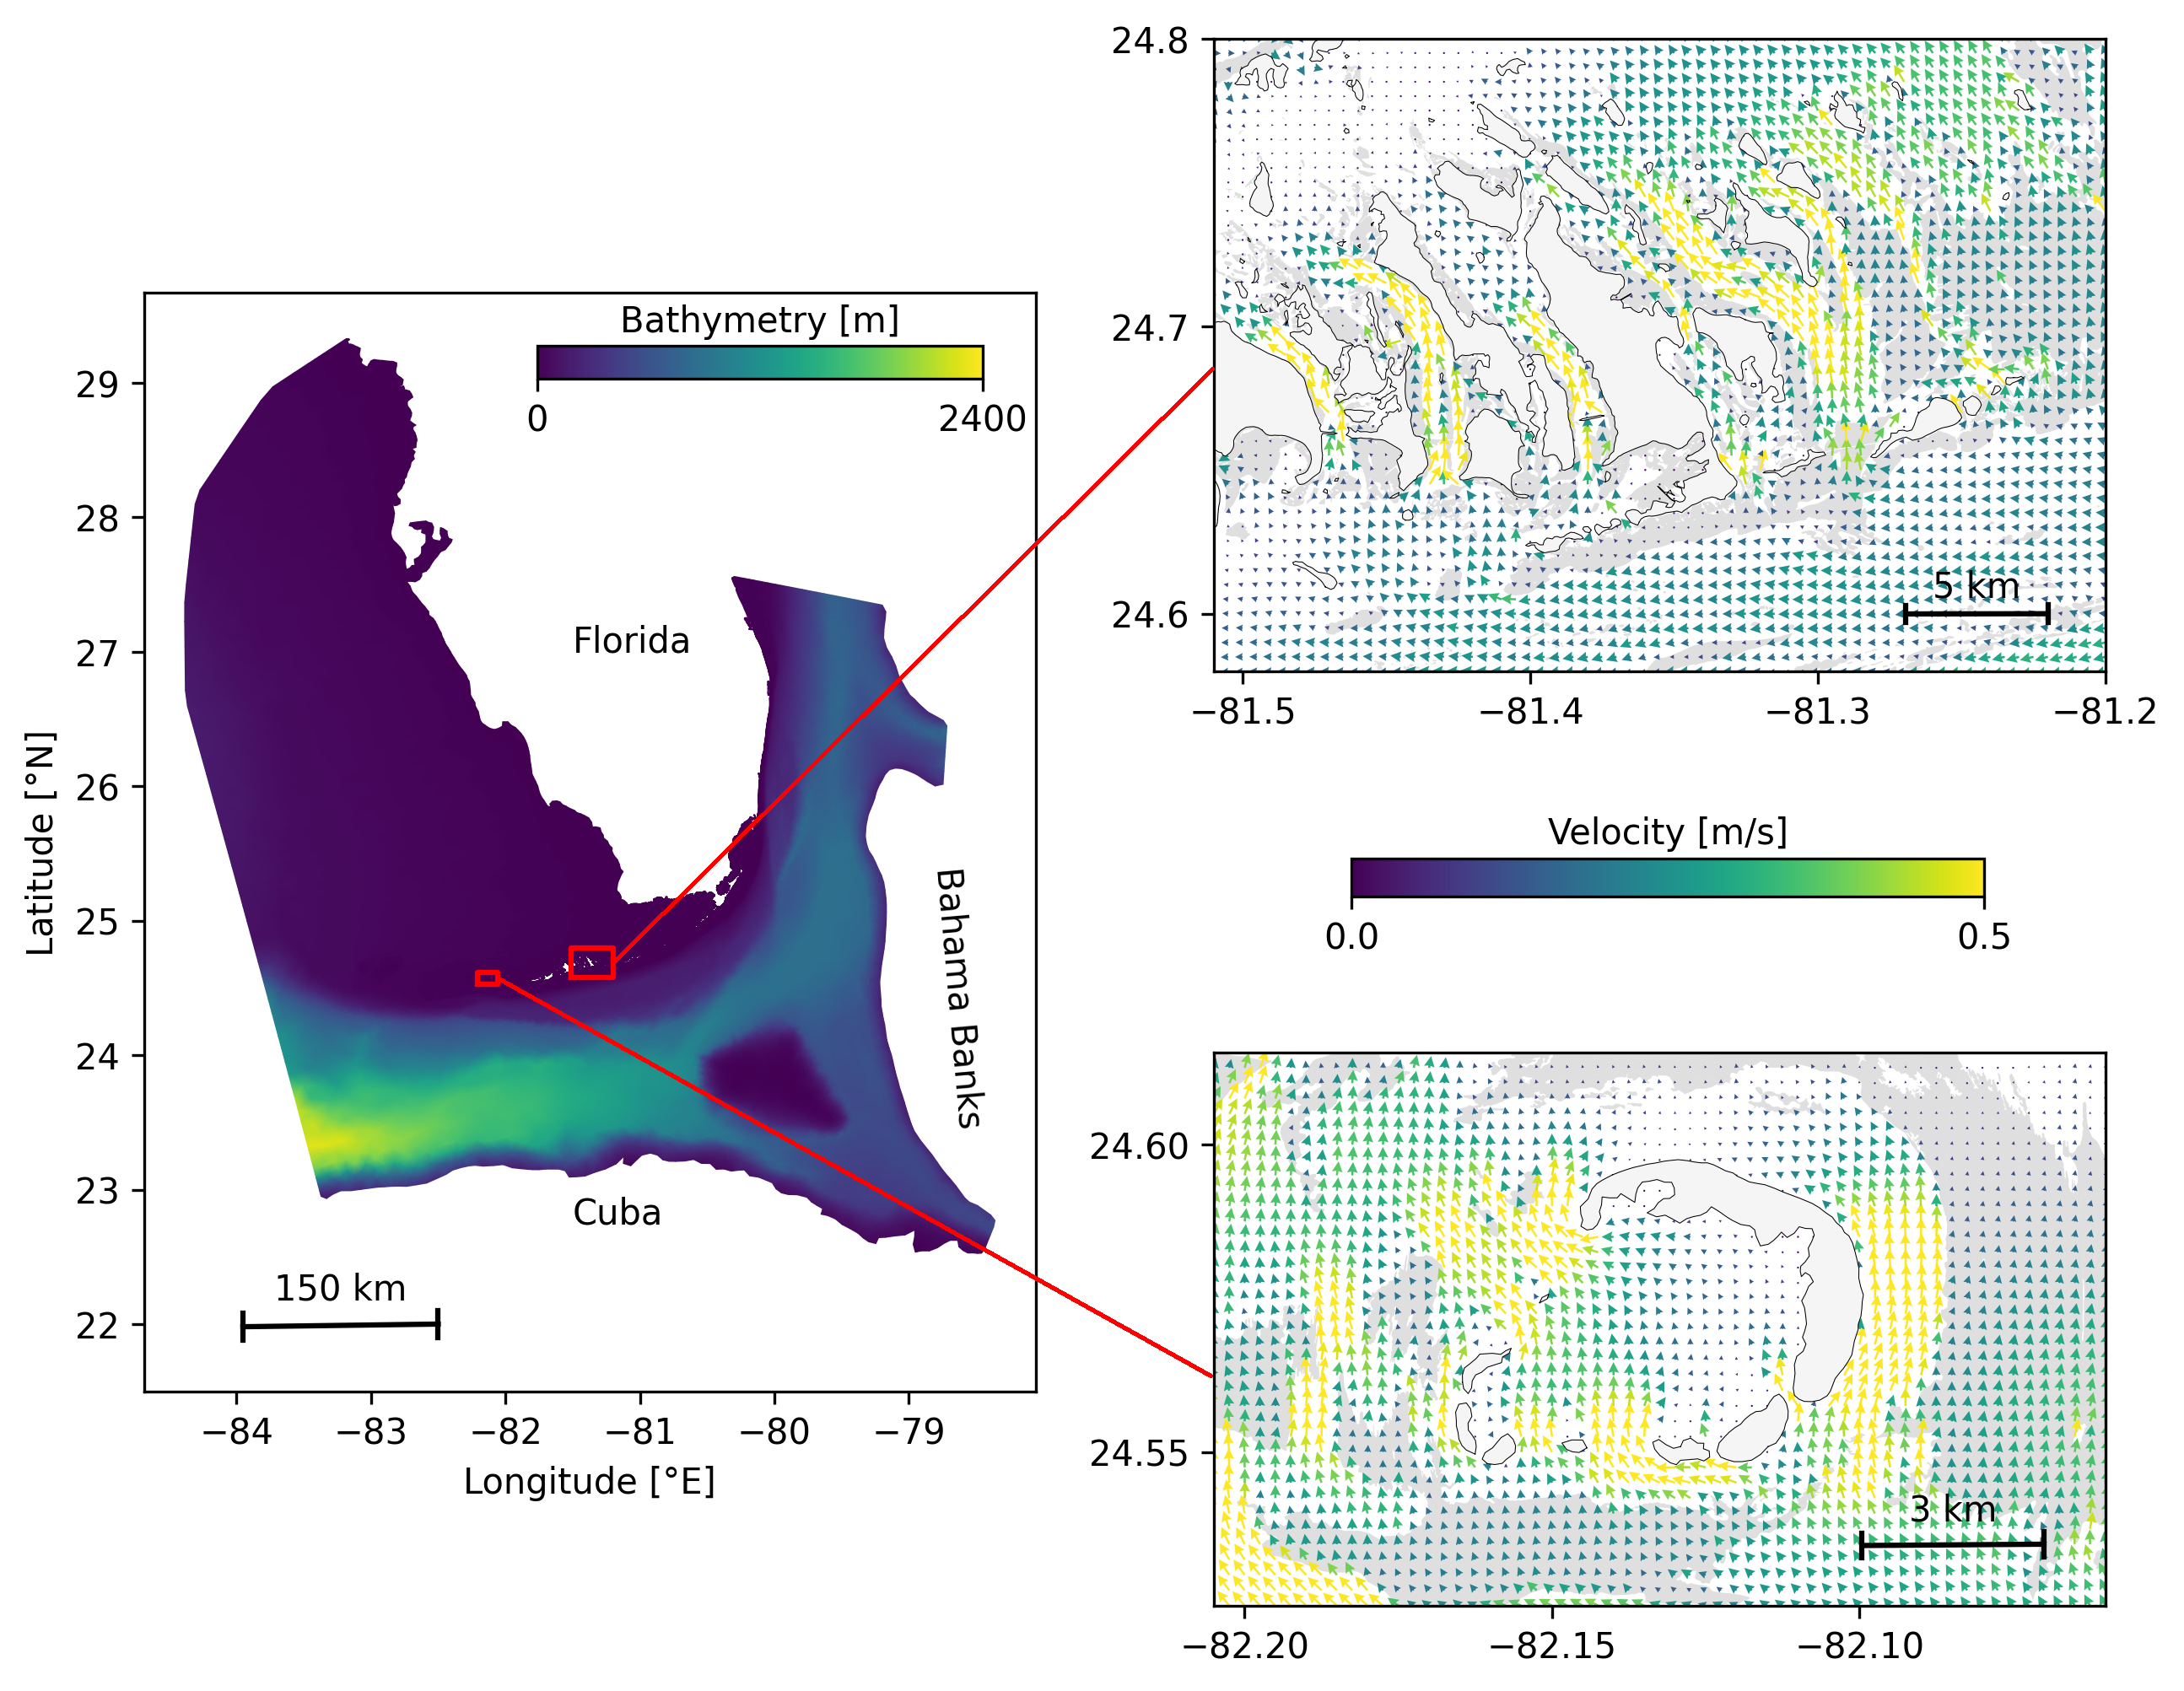
\includegraphics[width=.9\textwidth]{figures/setup_3.png}
    \caption{Model computational domain with the bathymetry (left) and close-up views of the mesh with snapshots of the currents on May, 25 2018 at 00:00, for the Marquesas Keys (bottom) and the Lower Keys (top). This illustrates the benefits of unstructured meshes to represent the fine-scale details of the topography and hence simulate currents down to the scale of individual reefs (shown in light grey) and islands (shown in white).}
    \label{fig:setup}
\end{figure}

The mesh resolution depends only on the distance to the coast but we distinguish between the coastlines along the FRT where we impose a maximum resolution of 100 m and the other coastlines along which the maximum resolution is 2500 m. The mesh has been generated with the open-source mesh generator GMSH \citep{Geuzaine2009} and has about $7 \times 10^5$ elements. The coarsest elements, far away from the FRT, have a size of about 10 km. An illustration of ocean currents simulated on that mesh are shown in Fig. \ref{fig:setup}. It shows how a 100-m spatial resolution allows us to simulate fine-scale details of the flow, such as recirculation eddies and currents within the dense reef system in the Lower Keys that consist of many individual reefs with narrow passages in between. 

The simulated currents can then be used to model dispersal of infectious material throughout the FRT. In this study, 3 types of potential vector carrying the disease causative agent were considered: positively buoyant (e.g. mucus and surfactant), neutrally buoyant (e.g. fines, pelagic organisms) and negatively buoyant (e.g. sediments, composites, demersal organisms). As SLIM is a depth-averaged model, the mean currents it generates are well suited to model the dispersal of neutrally buoyant material remaining within the water column. However, these currents must be modified to correctly represent the dynamics of materials evolving in the surface and bottom boundary layers. Therefore, surface current response to winds is estimated by adding 1.5\% of the wind speed to SLIM currents with a windage angle of 45$^\circ$ to the right for positively buoyant particles. Such parametrization is shown to be an accurate approximation of wave-induced Stokes drift and quasi-Eulerian surface currents by \citep{ardhuin2009observation}. For negatively buoyant materials, on the other hand, bottom currents are obtained by taking 60\% of SLIM currents velocity with a veering angle of 15$^\circ$ to the left. \lew{[Some references about the parametrizationfor bottom currents]}

Using these three velocity fields, virtual particles are then released on all the reefs composing the FRT to model the dispersal of infected materials carrying the disease causative agent. The locations of the reefs of Florida are extracted from the "coral reefs and hardbottom" layer of the Unified Florida Reef Tract Map \citep{fwc2017unified}. The polygon of this reef map are then further divided into 500 m squares in order to track the propagation of the disease with a finer geographical resolution, generating a total of 16823 polygons. % \textcolor{red}{(14058 without the big Vaca reef)}
At the beginning of each simulated months and for each type of currents, a total of about $1.5 \times 10^6$ particles are released over all the reef polygons. These particles have a state composed of their polygon of origin as well as their mass, initialized to 1, that they loose at a constant rate $\gamma$ as they are moved by surface, mean or bottom currents. In this study, the value of $\gamma$ is chosen so that particles have a half life of 30 days. When the particles are brought over reef polygons by currents, the amount of infected mass that lands on the polygon is recorded in monthly potential connectivity matrices whose entries are denoted $C_{ij}$. The matrix rows correspond to the source reefs and the columns correspond to the destination reefs. Hence $C_{ij}$ represents the mass of infected material originating from sub-reef i that has settled on sub-reef j. This matrix is then normalized by dividing each of its rows $i$ by the the total mass of particles released on polygon $i$ in order to obtained the normalized potential connectivity matrix $\tilde{C}$, whose entry $\tilde{C}_{ij}$ gives the probability that infectious material produced on sub-reef $i$ settles on sub-reef $j$. Connectivity matrices are computed for each type of current and for each month of the simulated period.

These connectivity matrices can be more easily handled by interpreting them as large graphs whose vertices are reefs. Such networks can then be analyzed using graph theory tools. In this study, 4 potential connectivity measures are used to interpret our monthly computed networks. These indicators are described in Table \ref{tab:indicator}. The first computed indicator is the weighted connectivity length (WCL), that gives the average dispersal distance from origin to destination for material produced on a given reef. The weighted connectivity of reef polygon $i$ writes:
\begin{equation}
    WCL_i = \dfrac{\sum_j \tilde{C}_{ij} L_{ij}}{\sum_j \tilde{C}_{ij}}
\end{equation}
where $L_{ji}$ is the distance between origin reef $i$ and destination reef $j$. Another measure of the spreading potential of reef $j$ is its out-degree, \ie the number of connections originating from reef $j$ in the network. This indicator is obtained by computing the number non-zero entries of row $i$ of the potential connectivity matrix $\tilde{C}$. The information given by the out-degree is complemented by the proportion of infectious elements produced on reef $i$ that successfully settles on a reef, called the fraction exchanged of reef $i$. This indicator is given by $\sum_{j} \tilde{C}_{ij}$. Finally, the isolation of reef $i$ in the network is given by the self recruitment, \ie the proportion of infectious matter settling on reef $i$ that originates from reef $i$, computed by $C_{ii}/\sum_jC_{ji}$. A large self-recruitment value indicates that few infectious matter produced elsewhere settles on the reef and thus that it is isolated from the rest of the network. 

\begin{table}
    \centering
    \begin{tabular}{|p{4cm}|p{5cm}|p{4cm}|}
        \hline
        \textbf{Indicators} & \textbf{Description} & \textbf{What it shows} \\
        \hline
            Weighted connectivity length (WCL) & 
            Average dispersal distance from origin to destination reef for all infectious elements released over a reef & 
            Average distance at which a reef can send infectious matter \\
        \hline
            Out-degree &
            Number of out-going connections originating from a given reef &
            Potential for a reef to spread the disease \\
        \hline
            Fraction exchanged &
            Fraction of infectious material produced on a given reef that settles on another reef &
            Success rate of potential disease spread  \\
        \hline
            Self recruitment &
            Fraction of infectious material settling on a given reef that has been released on the same reef &
            Potential for disease to settle on a given reef \\
        \hline            
    \end{tabular}
    \caption{Indicators used to analyze the modeled exchanges of infected material for each considered type of currents and for each simulated month}
    \label{tab:indicator}
\end{table}

% --> Subsection 2
\subsection{Epidemiological modeling}

\subsubsection{Model equations}

The spread of the SCTLD throughout the FRT is simulated using a connectivity-based Kermack-McKendrick SIR model \citep{brauer2008compartmental}. SIR models are among the most standard epidemiological models. They divide individuals into three compartments: susceptible (S), infectious (I) and removed (R). When affected by the disease, susceptible individuals become infectious and infect other susceptible individuals until they are removed, either by recovery or death. Such models usually rely on the hypothesis of an homogeneous, well-mixed population. To account for the spatial heterogeneity of the FRT, the basic SIR formulation is here modified by considering the proportions of susceptible ($S_j$), infectious ($I_j$) and removed ($R_j$) corals of each polygon reef $j$. In this epidemiological model, individual reefs interact through the exchange of infectious material as represented by the connectivity matrix. For each sub-reef $j$ and at any time, the following relations hold: $0\leq S_j,I_j,R_j\leq 1$ and $S_j+I_j+R_j=1$. The evolution of these proportions through time is governed by the following equations:
\begin{equation}
    \begin{aligned}
        \dfrac{dS_j}{dt} &= -\beta\sum_i\dfrac{A_i}{A_j}I_i\tilde{C}_{ij}S_j - \beta'(I_j)S_jI_j \\
        \dfrac{dI_j}{dt} &= \beta\sum_i\dfrac{A_i}{A_j}I_i\tilde{C}_{ij}S_j + \beta'(I_j)S_jI_j - \sigma I_j \\
        \dfrac{dR_j}{dt} &= \sigma I_j
    \end{aligned}\label{eq:epidemio}
\end{equation}
where $\tilde{C}_{ij}$ is the entry of reef $(i,j)$ of the normalized potential connectivity matrix [-], $A_i$ is the area of reef polygon $i$ [km$^2$], $\sigma$ is the removal rate [day$^{-1}$], and $\beta$ and $\beta'(I_j)$ are the inter- and intra-reef disease transmission rates [day$^{-1}$], respectively. In this model, infectious corals of reef $i$ can infect corals of reef $j$ if there is non-zero probability of infectious material exchange from reef $i$ to reef $j$, given by $\tilde{C}_{ij}$. Moreover, to account for coral resistance to the disease, the intra-reef transmission function $\beta'(I_j)$ has the shape of a smooth step function of the proportion of infectious corals $I_j$ and writes:
\begin{equation}
    \beta'(I_j) = \dfrac{\beta_0'}{2}(1+\tanh[(I_j-I_0)/\tau]),\label{eq:beta}
\end{equation}
where $I_0$ is a threshold on the infection population above which intra-reef transmission becomes significant, and $\tau$ is a measure of the interval over which the transition for low to high transmission occurs. As long as the proportion of infectious corals on reef $j$ is below $I_0$, the only infection mechanism taking place is connectivity-driven transmission at rate $\beta$. Once the threshold is exceeded ( $I_j \geq I_0$ ), intra-reef transmission with rate $\beta'_0$ is activated. A larger value of threshold $I_0$ corresponds to a greater resistance to disease for corals and therefore a slower spread of the disease within reef $j$. Coral birth and natural (\ie non SCTLD-related) death rates are not take into account in this model, as they are assumed to balance each other. This assumption seems reasonable since coral populations of the FRT were declining prior to the emergence of the SCTLD outbreak. For this study the same values were used for $\beta$ and $\beta'_0$.

\subsubsection{Calibration}

Transmission and removal parameters of $\sigma$ and $\beta_0'$ are fitted to disease prevalence observations averaged over all colonies from all monitored sites in the FRT in order to accurately simulate the temporal evolution of $S_j,I_j,R_j$ on each infected reef polygon. \erinn{[some details about parameter estimations from the meta-analysis would be nice here]}
To relate our model framework to the compiled data, Eqs $\ref{eq:epidemio}$ are simplified to a single-reef SIR system:
\begin{equation}
    \begin{aligned}
        \dfrac{dS}{dt} &= -\beta'_0SI \\
        \dfrac{dI}{dt} &= \beta'_0SI - \sigma I \\
        \dfrac{dR}{dt} &= \sigma I
    \end{aligned}\label{eq:simplified}
\end{equation}
Due to the low values of the entries of the normalized connectivity matrix $\tilde{C}_{ij}$, intra-reef transmission, when activated, is the dominant infection mechanism of Eq. \ref{eq:epidemio}. Consequently, Eqs. \ref{eq:simplified} give a reasonable approximation of the evolution of the disease on sub-reefs for which $I_j > I_0$. Using this approximation, the ratio $\beta_0'/\sigma$ is imposed by matching the modeled proportion of susceptible corals remaining after the disease has vanished ($S_\infty$) with observations. A standard property of a SIR model solution is that
\begin{equation}
    S_\infty - \frac{\sigma}{\beta_0'}\log(S_{\infty}/S_0) = 1\label{eq:ratio}
\end{equation}
where the initial proportion of susceptible corals is taken equal to $1-I_0$ (see for instance \cite{Murray07}). In the framework of Eqs. \ref{eq:simplified}, the ratio $\beta_0'/\sigma$ gives the value of the basic reproduction number $R_0$, defined as the average number of secondary cases produced by one
infected individual introduced into a population of susceptible individuals \citep{keeling2007stochastic}. This
number is used in epidemiological models to determine whether an emerging infectious disease can spread in a
population ($R_0 > 1$) or not ($R_0 < 1$). The obtained basic reproduction number is then used to find the value of $\beta'_0$ that reproduces the observed temporal evolution of the state of the coral colonies.

\subsubsection{Initialization}

In order to solve Eqs. \ref{eq:epidemio}, initial conditions are needed, \ie proportions of susceptible, infectious and recovered corals at the beginning of the simulated period. This information is constructed based on different field-collected datasets: : (i) Coral Reef Evaluation and Monitoring Project (CREMP; 2014–2017), (ii) CREMP Presence/Absence Data (CREMP P\_A; 2016–2017), (iii) Southeast Florida Coral Reef Evaluation and Monitoring Project (SECREMP; 2014– 2017), (iv) Florida Reef Resilience Program Disturbance Response Monitoring (FRRP; 2014–2017), (v) Hurricane Irma Rapid Reef Assessment (IRMA; 2017, \cite{viehman2018}), (vi) the Southeast Florida Action Network citizen science program (SEAFAN; 2014–2017), and (vii) the Southern Coral Disease Margin field effort (2017; \cite{neely2018surveying}). These datasets give the locations and dates at which the SCTLD has been observed throughout the FRT. Using this information, we first delineate an infected zone by constructing the concave hull of the points where the disease was observed before May 2018. The reefs infected prior to the beginning of our simulated period are then defined as the reefs located inside the constructed zone. The time of observed infection is then spatially interpolated on each reef of the infected zone by kriging with a Gaussian semivariogram using Python \texttt{pyKrige} module. Assuming an initial state $(S,I,R)=(1-I_0, I_0, 0)$ when the disease was observed, the proportions of susceptible, infectious and removed corals on each reef of the infected zone on the 1st May 2018 is finally approximated using the simplified equations \ref{eq:simplified}. Reefs outside of the infected zone are initialized with a population of 100\% of susceptible corals.  

\subsubsection{Computation of front speed}

\begin{figure}
    \centering
    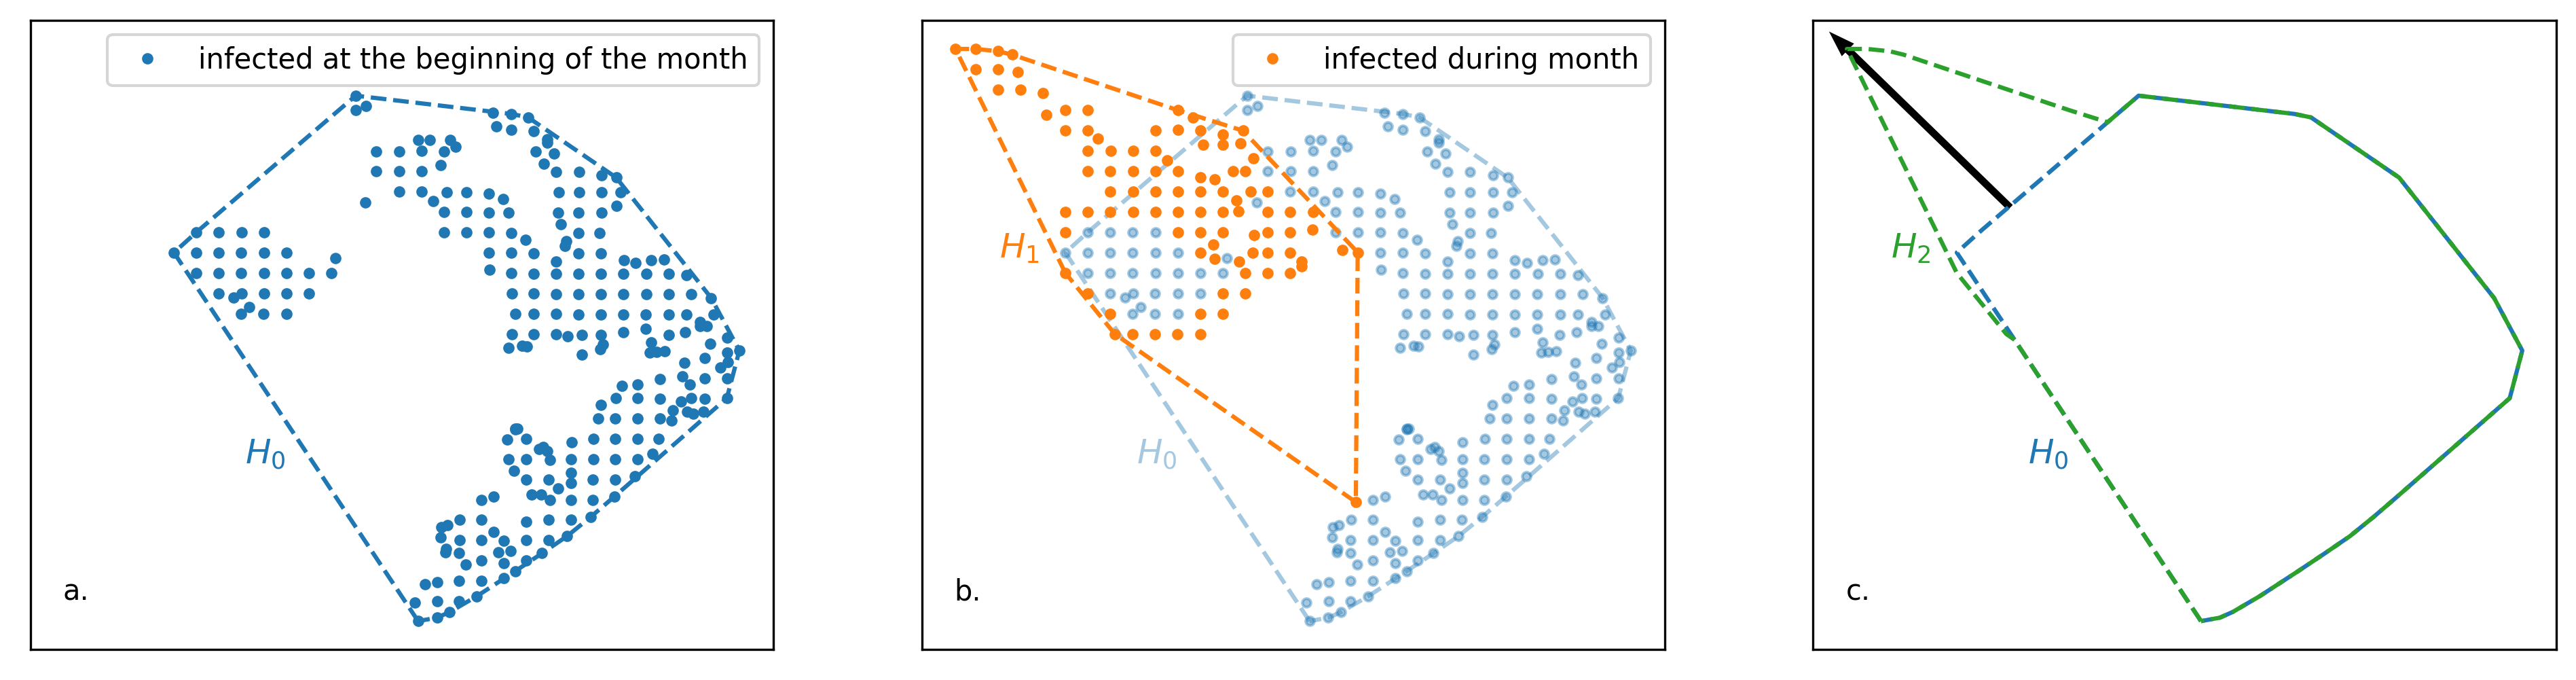
\includegraphics[width=.99\linewidth]{figures/hull_example.png}
    \caption{Method used to compute the disease front displacement during a simulated time interval.\textbf{a.} Concave hull of the infected polygons at the beginning of the simulated period $H_0$. \textbf{b.} Concave hull of the polygons infected during the simulated simulated $H_1$. \textbf{c.} Arrow showing the computed front displacement during simulated time interval between $H_0$ and $H_2$, the union of $H_0$ and $H_1$.}
    \label{fig:hull}
\end{figure}

\cite{muller2020spatial} estimated the speed of the spreading STCLD epidemics at around 92 m/day in the southern section of the FRT. In order to assess our simulation results in regard to this value, we developed a methodology to compute the displacement of the disease front during a given time interval within our simulatzd period. First, the concave hull of the infected polygons at the beginning of the time interval $H_0$ is computed. Then the concave hull of the polygons infected during the time interval $H_1$ is computed while the concave hull $H_2$ is defined as the union of $H_0$ and $H_1$. This methodology is illustrated in figure \ref{fig:hull}. The distance traveled by the disease front is then obtained by computing:
\begin{equation}
    \max\limits_{\mathbf{x}_2\in H_2}\min\limits_{\mathbf{x}_0\in H_0} \|\mathbf{x}_2 - \mathbf{x}_0\|_2
\end{equation}
The epidemics front speed is finally computed by dividing the resulting distance by the number of days in the simulated time interval.

%%%%%%%%%%%%%%%%%%%
% --- RESULTS --- %
%%%%%%%%%%%%%%%%%%%
\section{Results}

\subsection{Exchanges of infected materials}

The statistical behavior of the connectivity indicators used to analyze the monthly potential connectivity matrices for each type of currents are given in figure \ref{fig:connect}. Bottom currents exhibit the lowest dispersal potential as they generate the networks with the lowest weighted connectivity length and out-degree. However, infectious matters transported by bottom currents have the largest settlement success rate as these currents generate the graphs with the largest fraction exchanged. Therefore, bottom currents tend to transport more infectious material on fewer, closer reefs compared to the two other modes of transport.

Mean and surface currents, on the other hand show similar spreading ranges with mean WCL of 20.63 km and 21.39 km respectively. However, although surface currents tend to transport infectious elements on largest distances, these elements tend to settle on fewer reef, as these currents generate networks with smaller mean out-degree (321) than mean currents (416). Furthermore, the proportion of infectious material produced on reefs that successfully settles on a reef is on average 2.1\% with surface currents and 5.8\% with mean currents. Hence, although surface currents transport infectious matter on larger distances than mean barotropic currents, they tend to bring smaller amounts of infectious material on fewer reefs.

Self recruitment measures the isolation of the reefs in the network. Since infectious material is less likely to settle on isolated reefs, self recruitment measures the probability for the disease to settle on a given reef, whereas all three other indicators inform on the reef spreading potential. Fig. \ref{fig:connect} shows that the disease is more likely to settle on the reefs of networks generated by mean currents. This result is consistent with the values of the other connectivity measures, as reefs tend to be more strongly connected with mean currents. On the other hand, reefs are more isolated with bottom currents, as they produce the graphs with lowest WCL and out-degree. Finally, surface currents generate larger self recruitment values than mean currents as they exhibit the lowest fraction exchanged. 

\begin{figure}
    \centering
    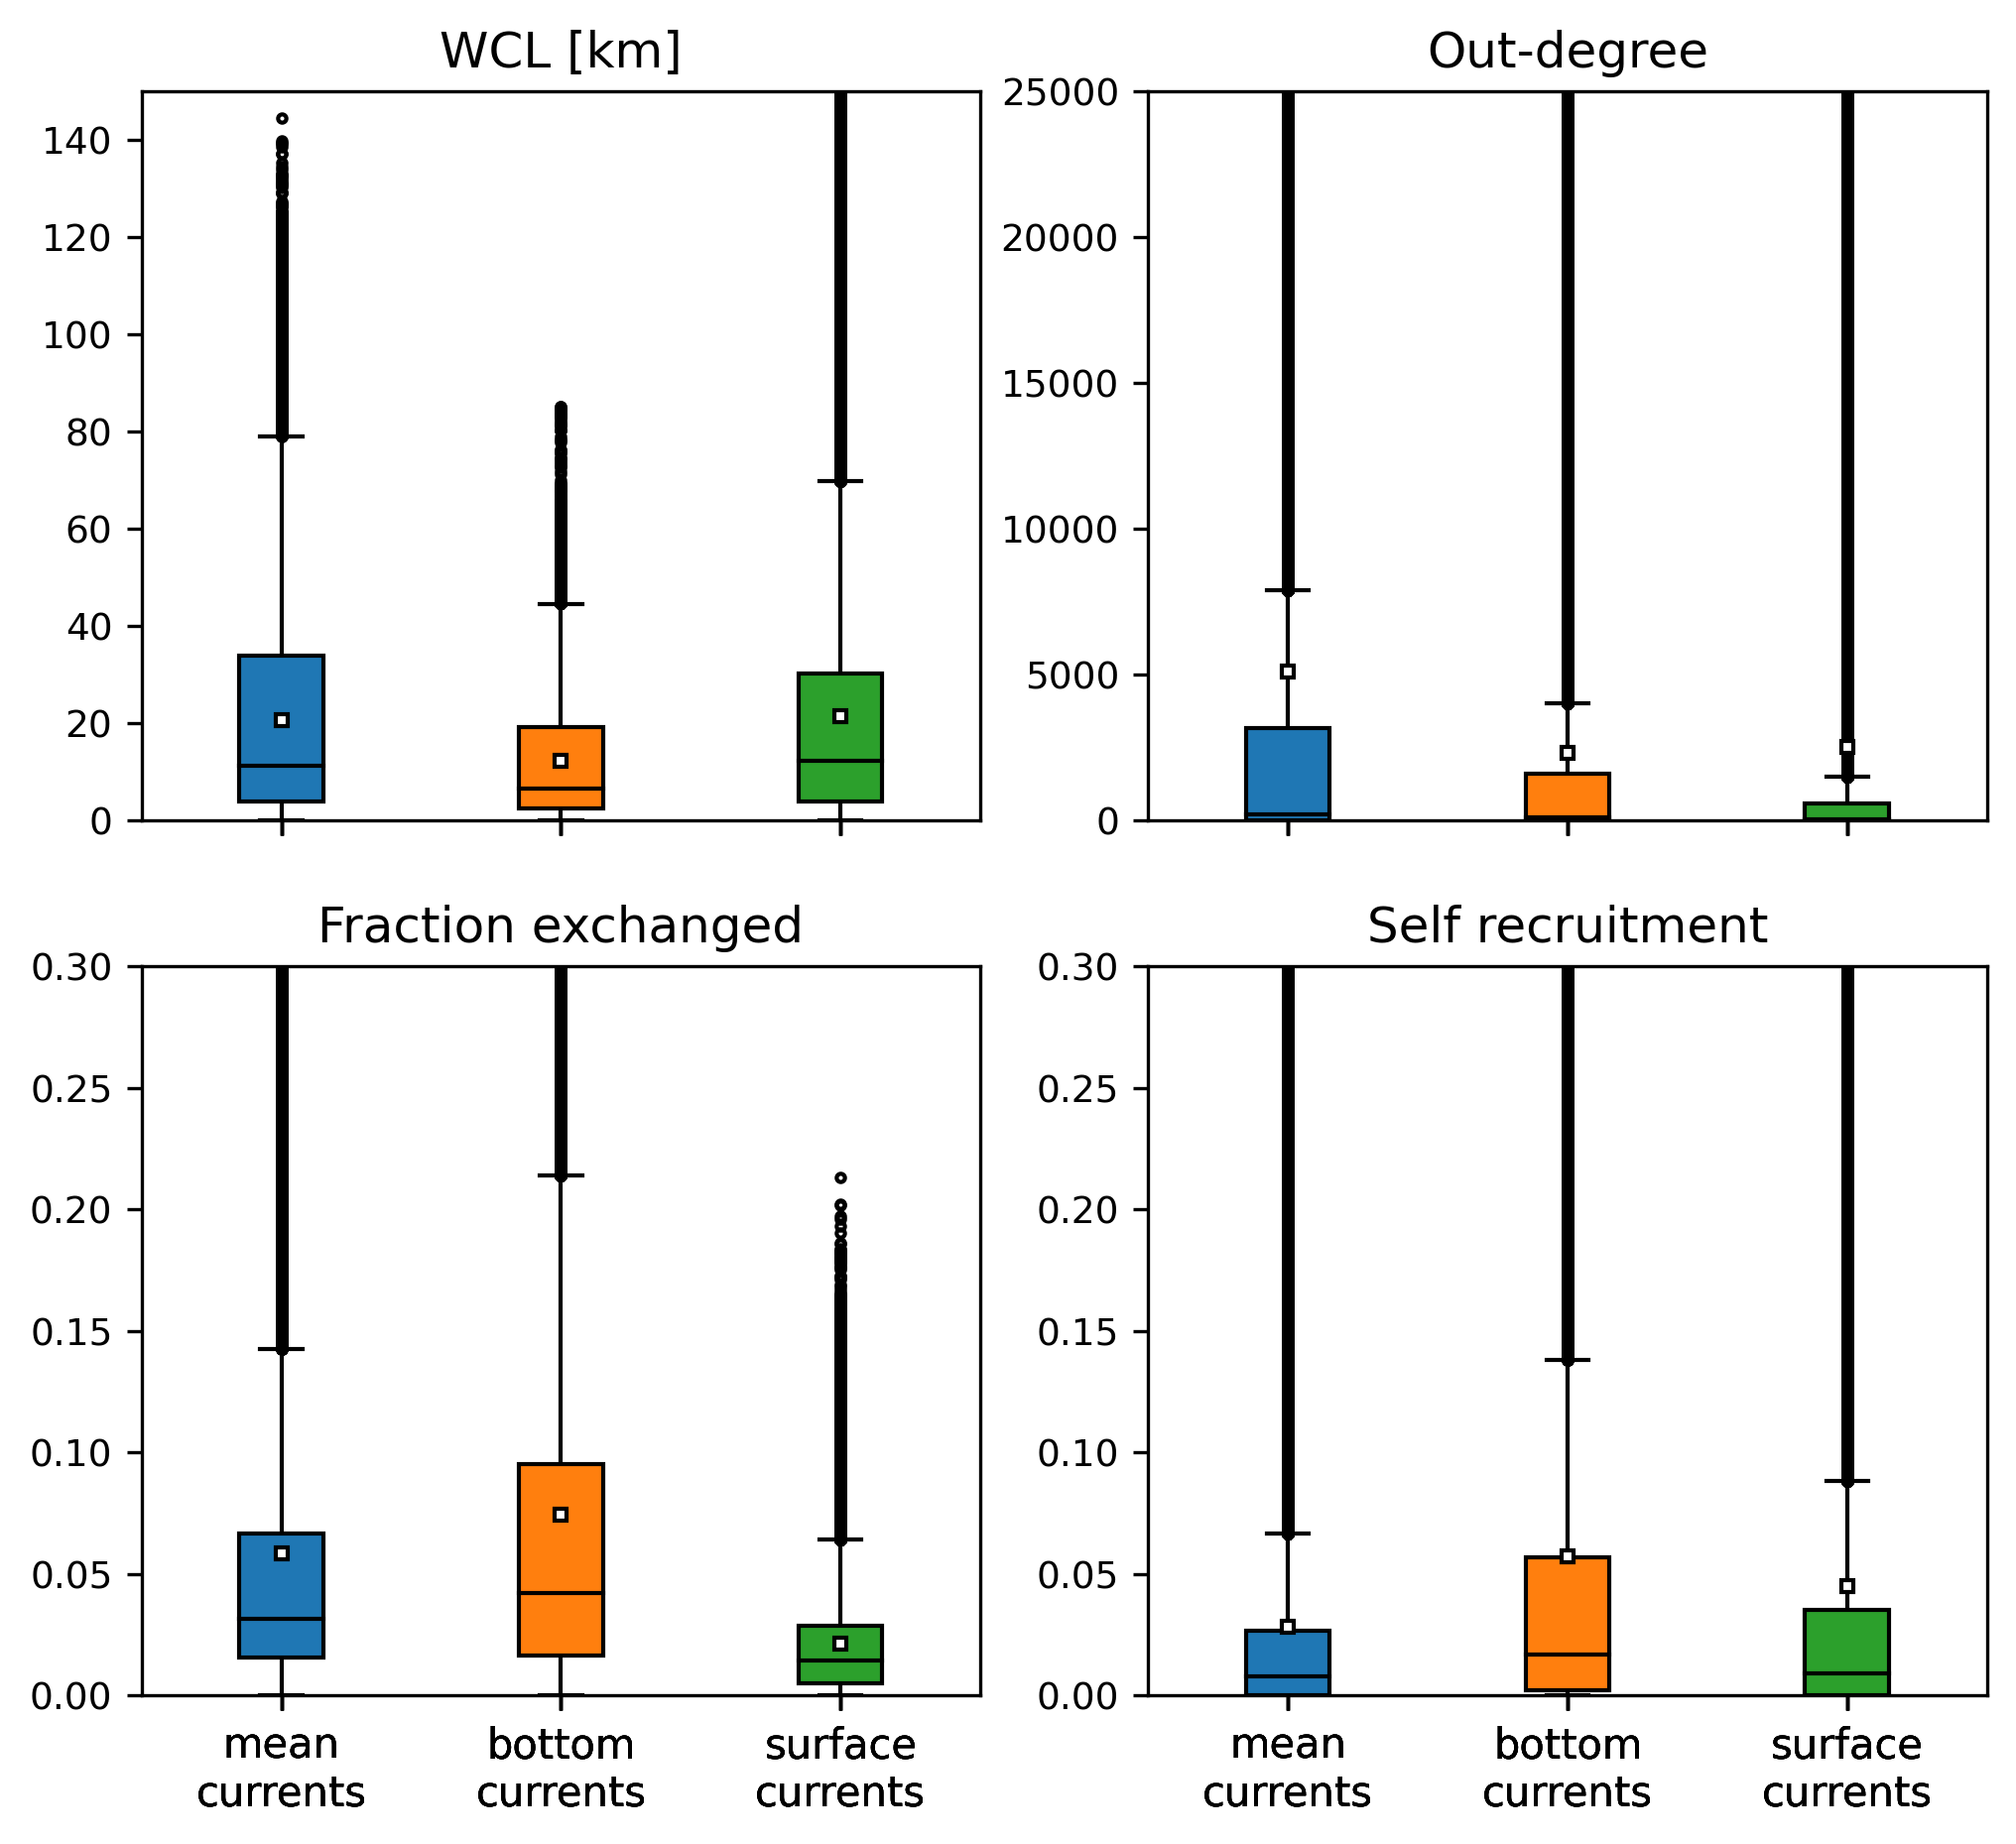
\includegraphics[width=.8\textwidth]{figures/connect_paper.png}
    \caption{Statistical behavior of the indicators derived from the monthly connectivity matrices computed for each type of current during our simulated period. Mean values are indicated by white squares}
    \label{fig:connect}
\end{figure}

\subsection{Epidemiological model results}

Best fit to averaged disease prevalence observations is obtained with transmission rate $\beta_0^{-1}'=6.45$ days and removal rate $\sigma^{-1}=6.99$ days. Comparison of the evolution of the state described by Eqs \ref{eq:simplified} results with observations is shown in figure \ref{fig:calibration}. Transmission and removal rates are found to have fairly close values with basic  $\beta_0'/\sigma$ being equal to $1.0345$. This proximity in rate values is imposed by Eq. \ref{eq:ratio}, as aggregated observations show a proportion of susceptible individuals of about $85\%$ at the end of the outbreak. Since infection and removal occur at very close rates, the instantaneous proportion of infectious individuals on the reefs remains pretty low through the outbreak, with a maximum value of about $0.4\%$.
\dobby{[I might come up with some more ideas when figures merged, as it will ease comparisons]}
%These results are in accordance with the characteristic infection time of $\sim 10.5$ days deduced from transmission experiments.

\begin{figure}
    \centering
    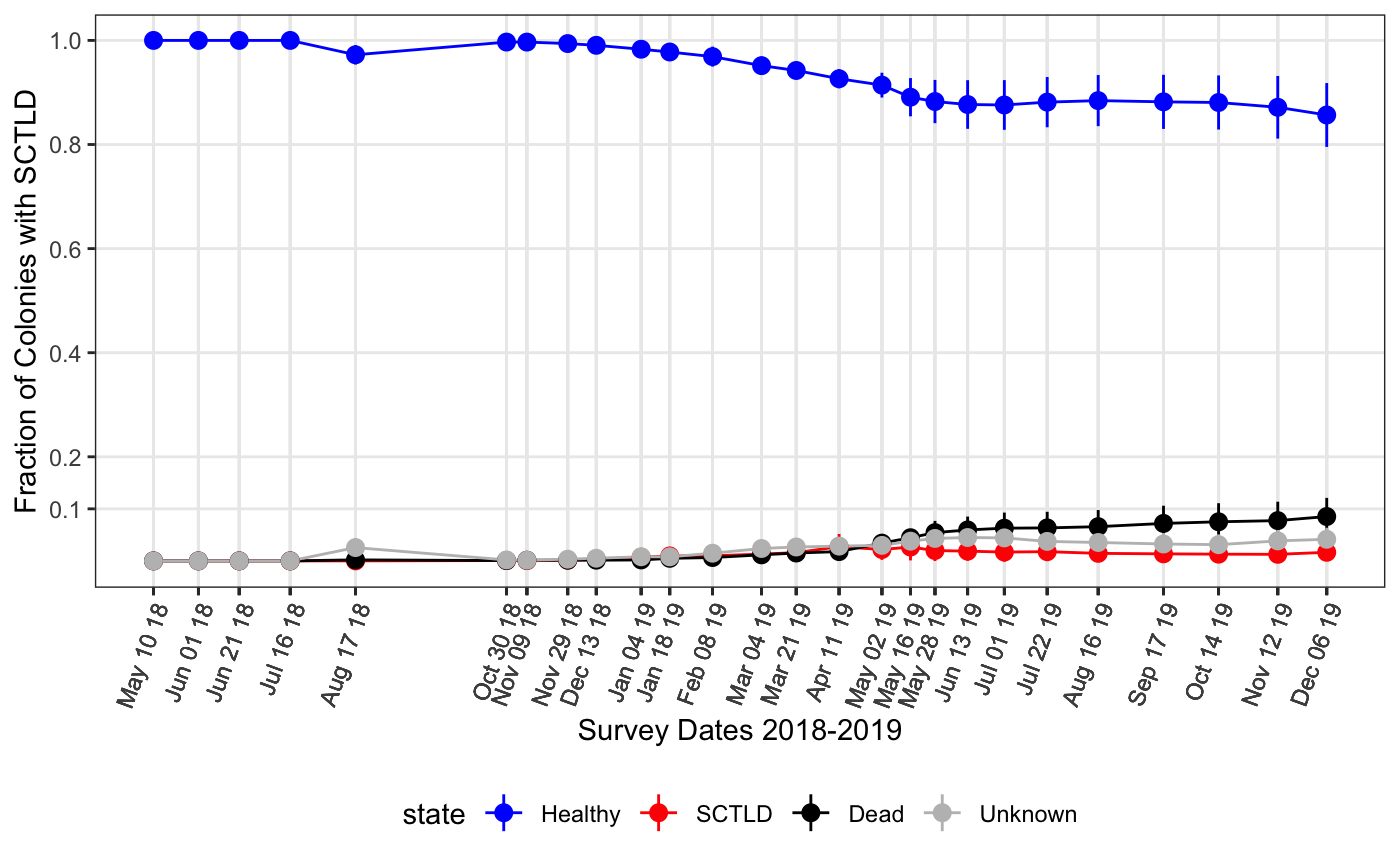
\includegraphics[width=.7\textwidth]{figures/image2.png}
    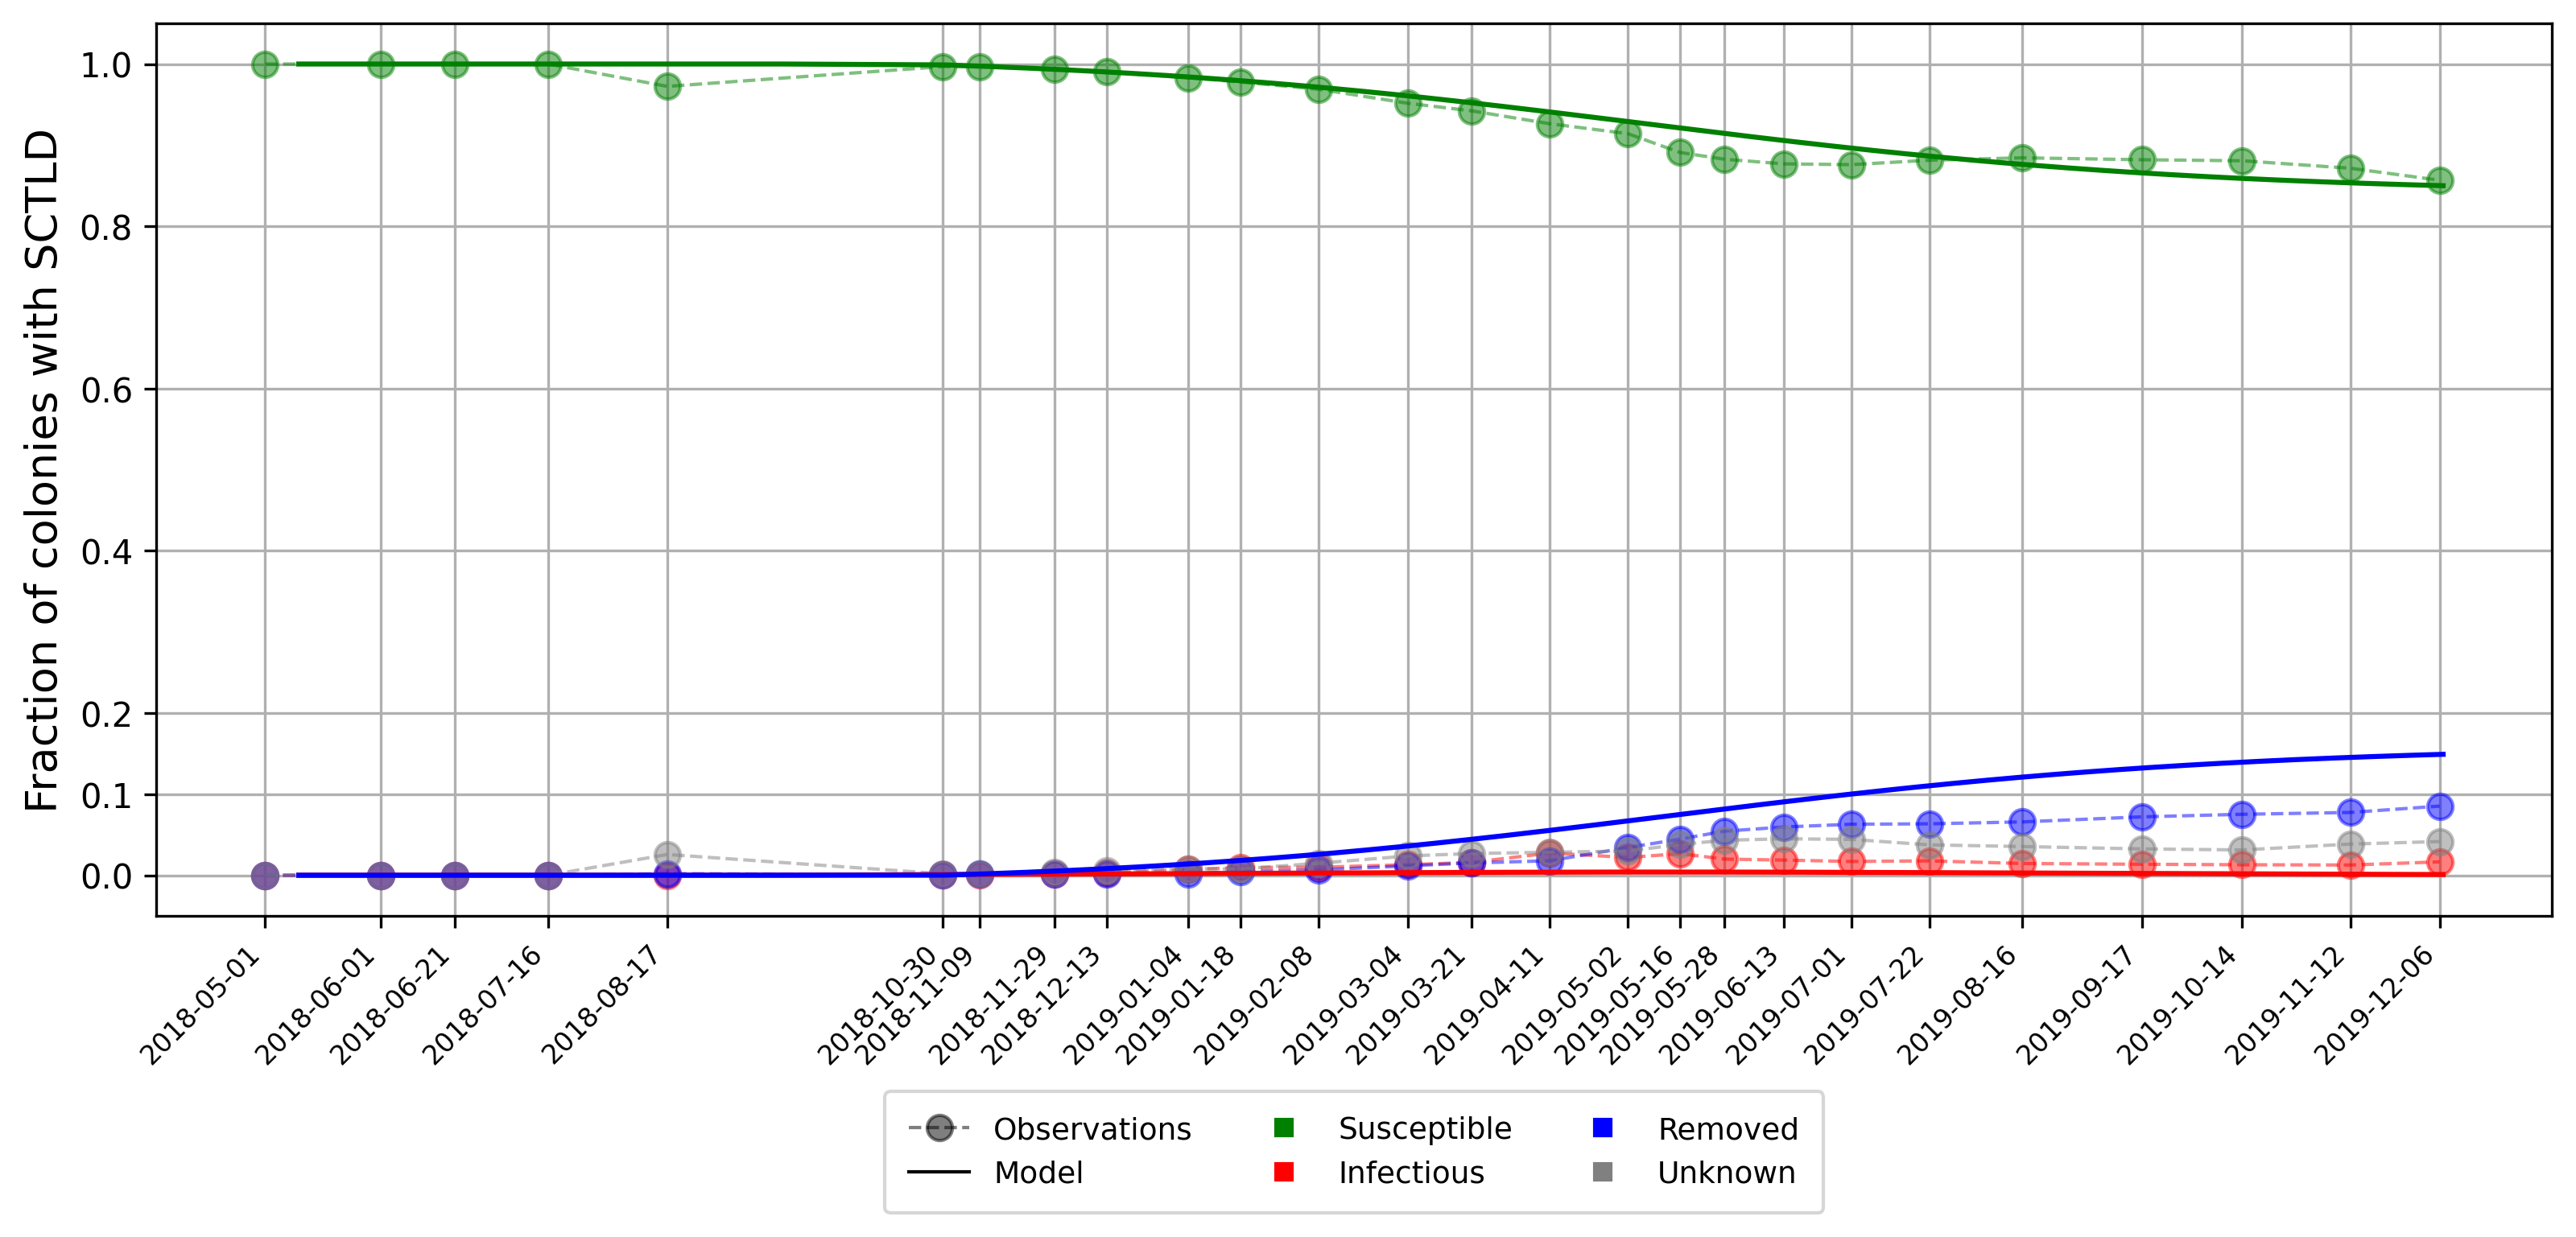
\includegraphics[width=.69\textwidth]{figures/sir_obs.png}
    \caption{\textbf{Above:} Observed disease prevalence over time (all colonies from all sites), error bars are the 95\% confidence intervals. \textbf{Below:} Disease prevalence over time as modeled by Eqs. \ref{eq:simplified} using calibrated transmission and removal parameters  $\beta_0^{-1}'=6.45$ days and $\sigma^{-1}=6.99$ days. \erinn{[data of the top figure]}}
    \label{fig:calibration}
\end{figure}

Using the above calibrated epidemiological parameters, epidemiological model simulations were performed from 1st May 2018 to 1st April 2019 for each type of currents and different values of the infection threshold $I_0$. A summary of the simulation results are shown in figure \ref{fig:results}. Two metrics are used to assess the accuracy of the model. First, the modeled front speed is compared to the reference rate of 92 m/day derived by \cite{muller2020spatial}. Furthermore, we computed the mean of the distances between each point where the SCTLD has been observed during our simulated period and the centroid of the closest reef polygon predicted to be infected by our model during the same period. These two indicators balance each other as scenarios that overestimate the front speed are more likely to predict infection near monitored reefs. Bottom currents produce the slowest modeled disease propagation with a maximum front speed of $\sim 20$ m/day, while simulations performed with surface currents spread the disease at a maximum speed of of about 60 m/day. However, surface currents tend to propagate the disease to the north, rather than westward, along the Florida Keys. This explains why bottom currents predict infection closer to observations despite exhibiting slower front speed. Finally, Mean barotropic currents outperform other types of current regarding both criteria with a front speed of 107 m/day and a mean geographical accuracy of $\sim1.2$ km. This suggest that the causative agent of the disease might be transported within neutrally buoyant material driven from reef to reef inside the water column by mean currents.

Moreover, Fig. \ref{fig:results} shows a strong dependence of model results to infection threshold $I_0$, that gives the proportion of infectious individual that colonies can withstand before exponential disease growth is triggered on reef. Front speeds of both mean and bottom currents reach a plateau for values of infection threshold between $I_0=0.05\%$ and $I_0=0.1\%$, while the minimal prediction error is attained around $I_0 \approx 0.078\%$ with mean currents. For $I_0 > 0.1\%$, intra-reef infection is strongly impeded and populations of infectious individuals on infected reefs are not able to become sufficiently large to infect other colonies on reefs they are connected to. For values of $I_0$ lower than $0.05\%$ on the other hand, intra-reef infection dominates and coral population on infected reefs is removed too fast to efficiently spread the disease through the network. Since disease propagation throughout the FRT only occurs for fairly small values of $I_0$ in our model, corals are expected to have low resistance to the causative agent of the SCTLD. 

\begin{figure}
    \centering
    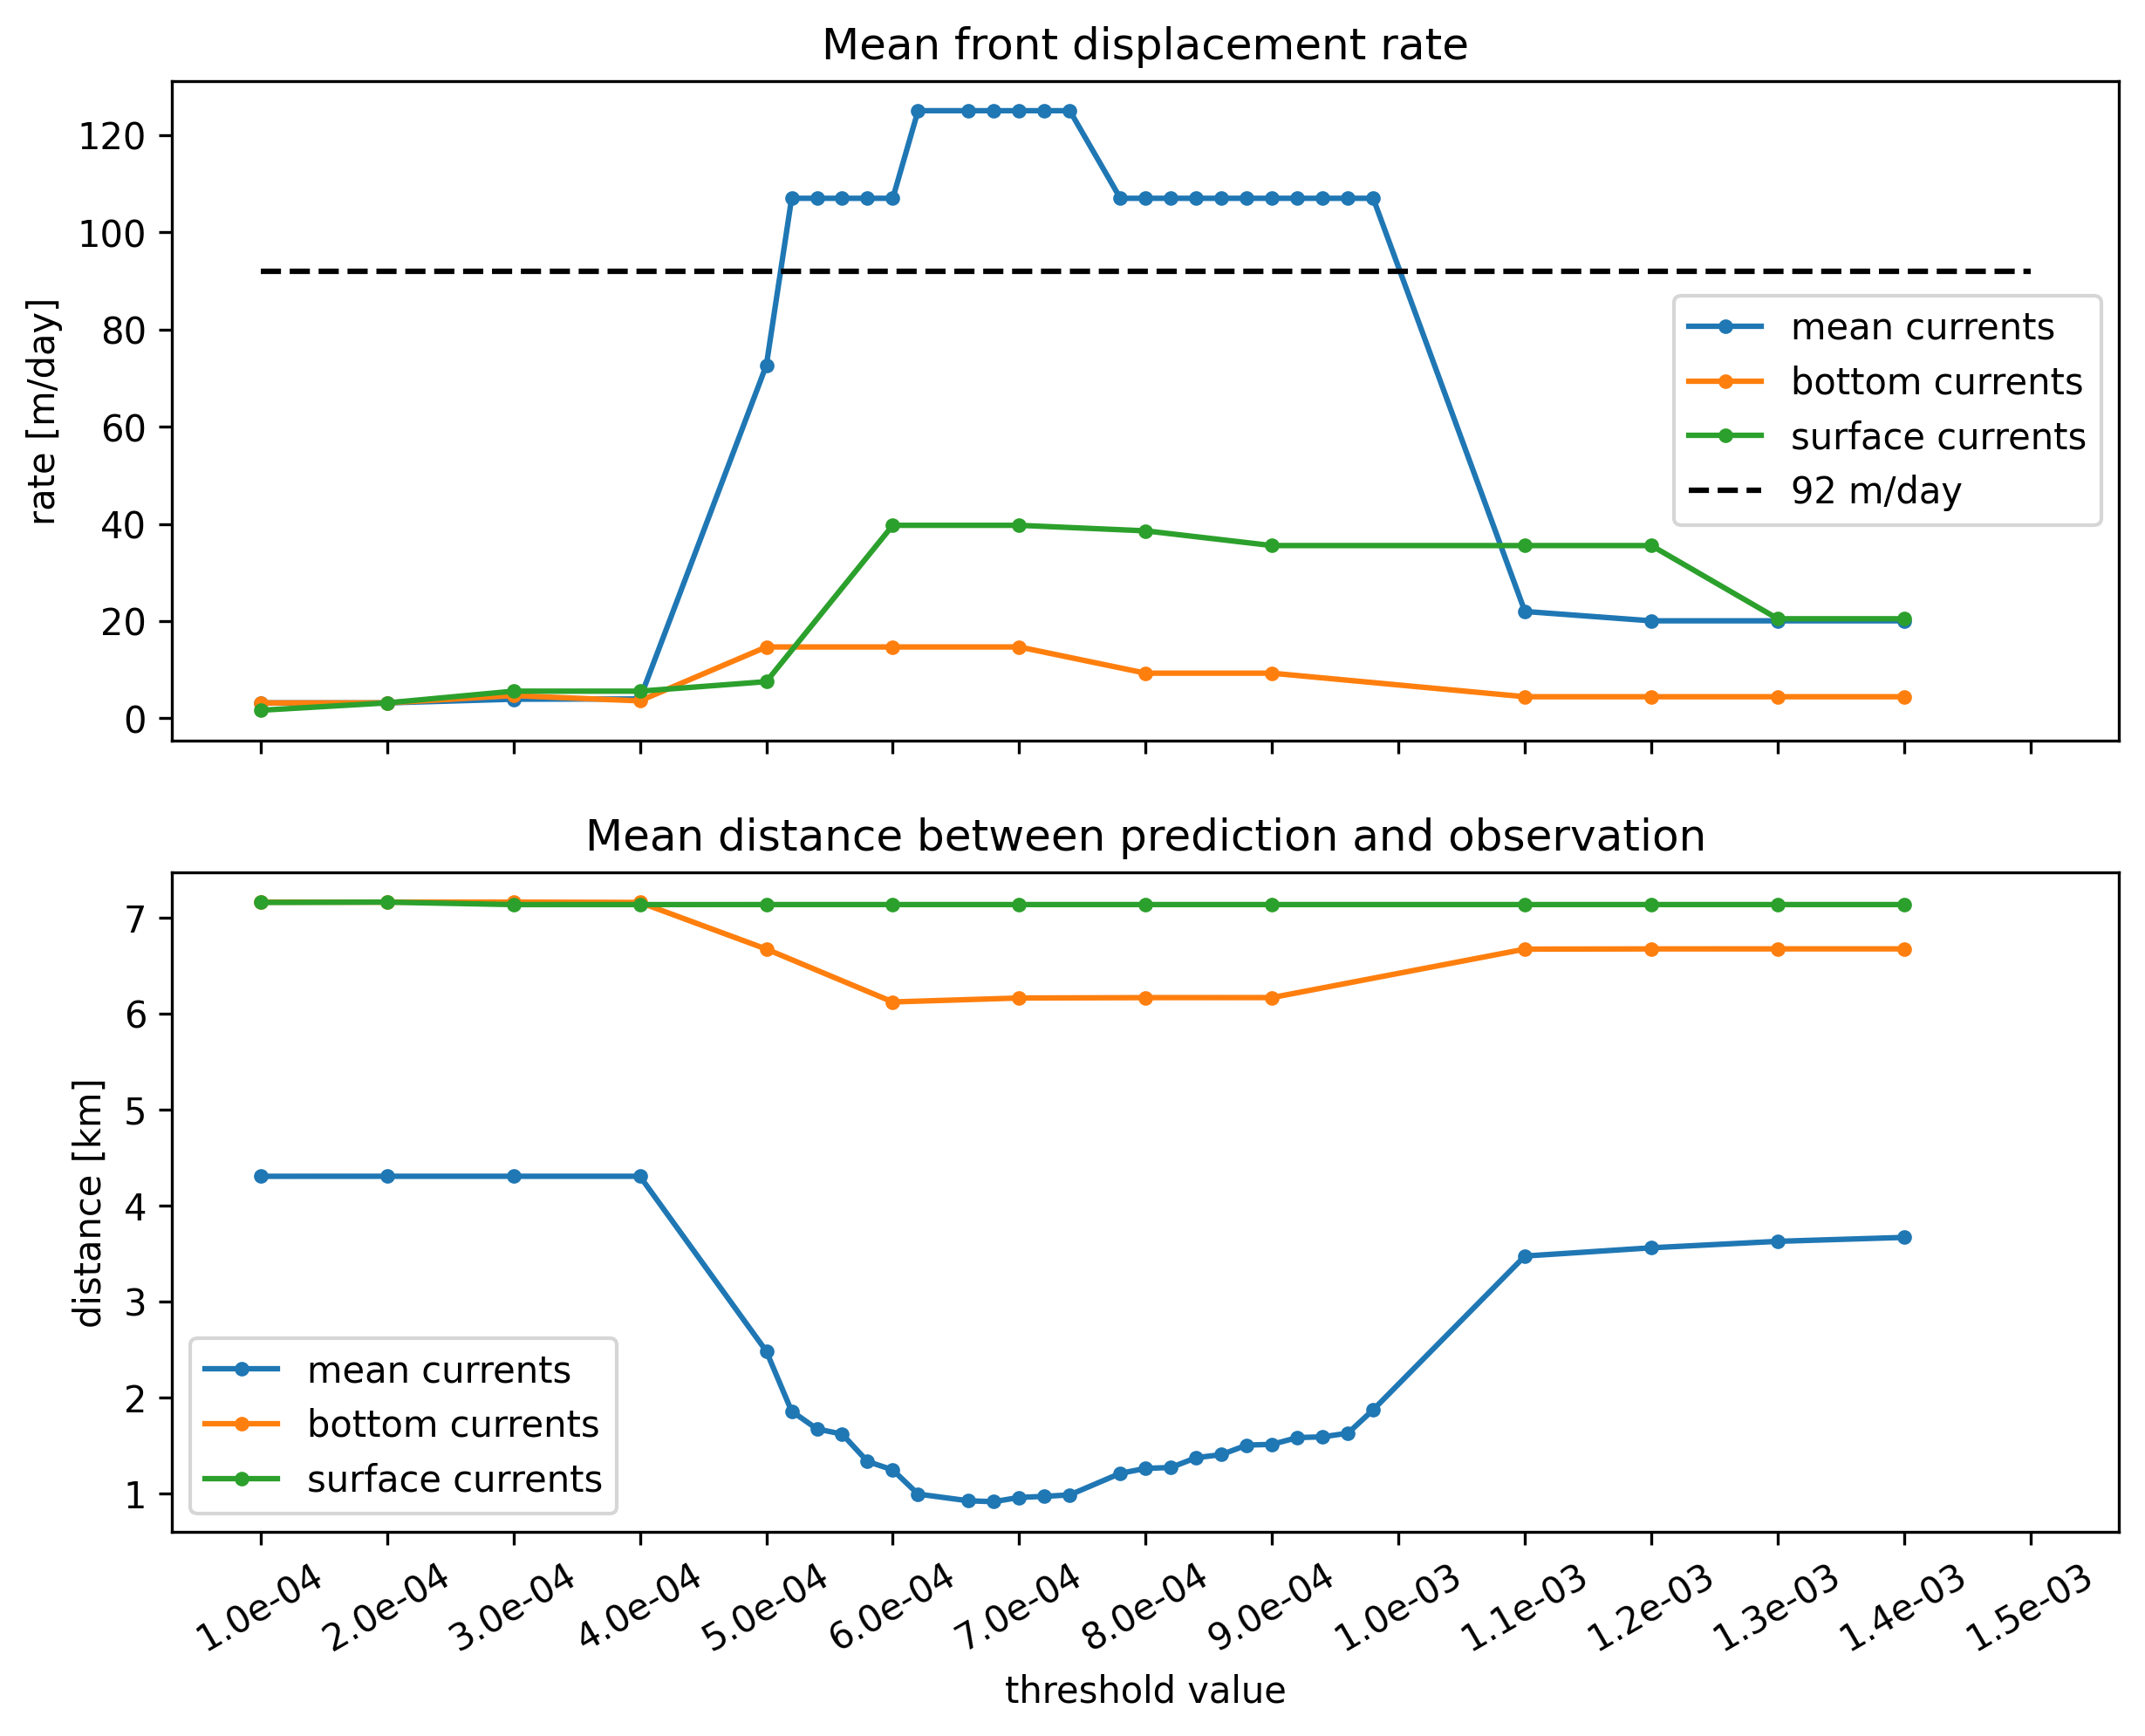
\includegraphics[width=.8\textwidth]{figures/sctld_validation_corrected.png}
    \caption{Summary of epidemiological model simulations with calibrated transmission parameters. \textbf{Top:} Modeled disease front speed for each type of current with respect to intra-reef infection threshold $I_0$. \textbf{Bottom:} Mean distance between predicted infected reefs and observed disease points. These results show that mean barotropic currents outperform other modes of transport at reproducing the observed spread of the disease. The appearance of a plateau suggests that model predictions are very sensitive to the value $I_0$}
    \label{fig:results}
\end{figure}

The results shown in figure \ref{fig:results} were obtained by removing the large reef located North to Vaca key, denoted Vaca reef as in \cite{frys20}, from our reef polygons. Preliminary simulations showed that this reef has close to no impact on the modeled spread of the disease to the rest of the FRT, as it sends few infectious matters to southerly and easterly neighboring reefs. Moreover, Vaca reef has a low coral coverage ($0-10\%$), which strongly impedes disease spread on the reef. However, as coral coverage is not taken into account in our epidemiological model, propagation of the disease on the reef was overestimated. This led to unrealistically strong modeled front speed variations due to the large size of the reef. Consequently, and in the absence of SCTLD observations on Vaca reef, it has been removed from our reef polygons in order to avoid overestimation of the disease spread.

% \begin{figure}
%     \centering
%     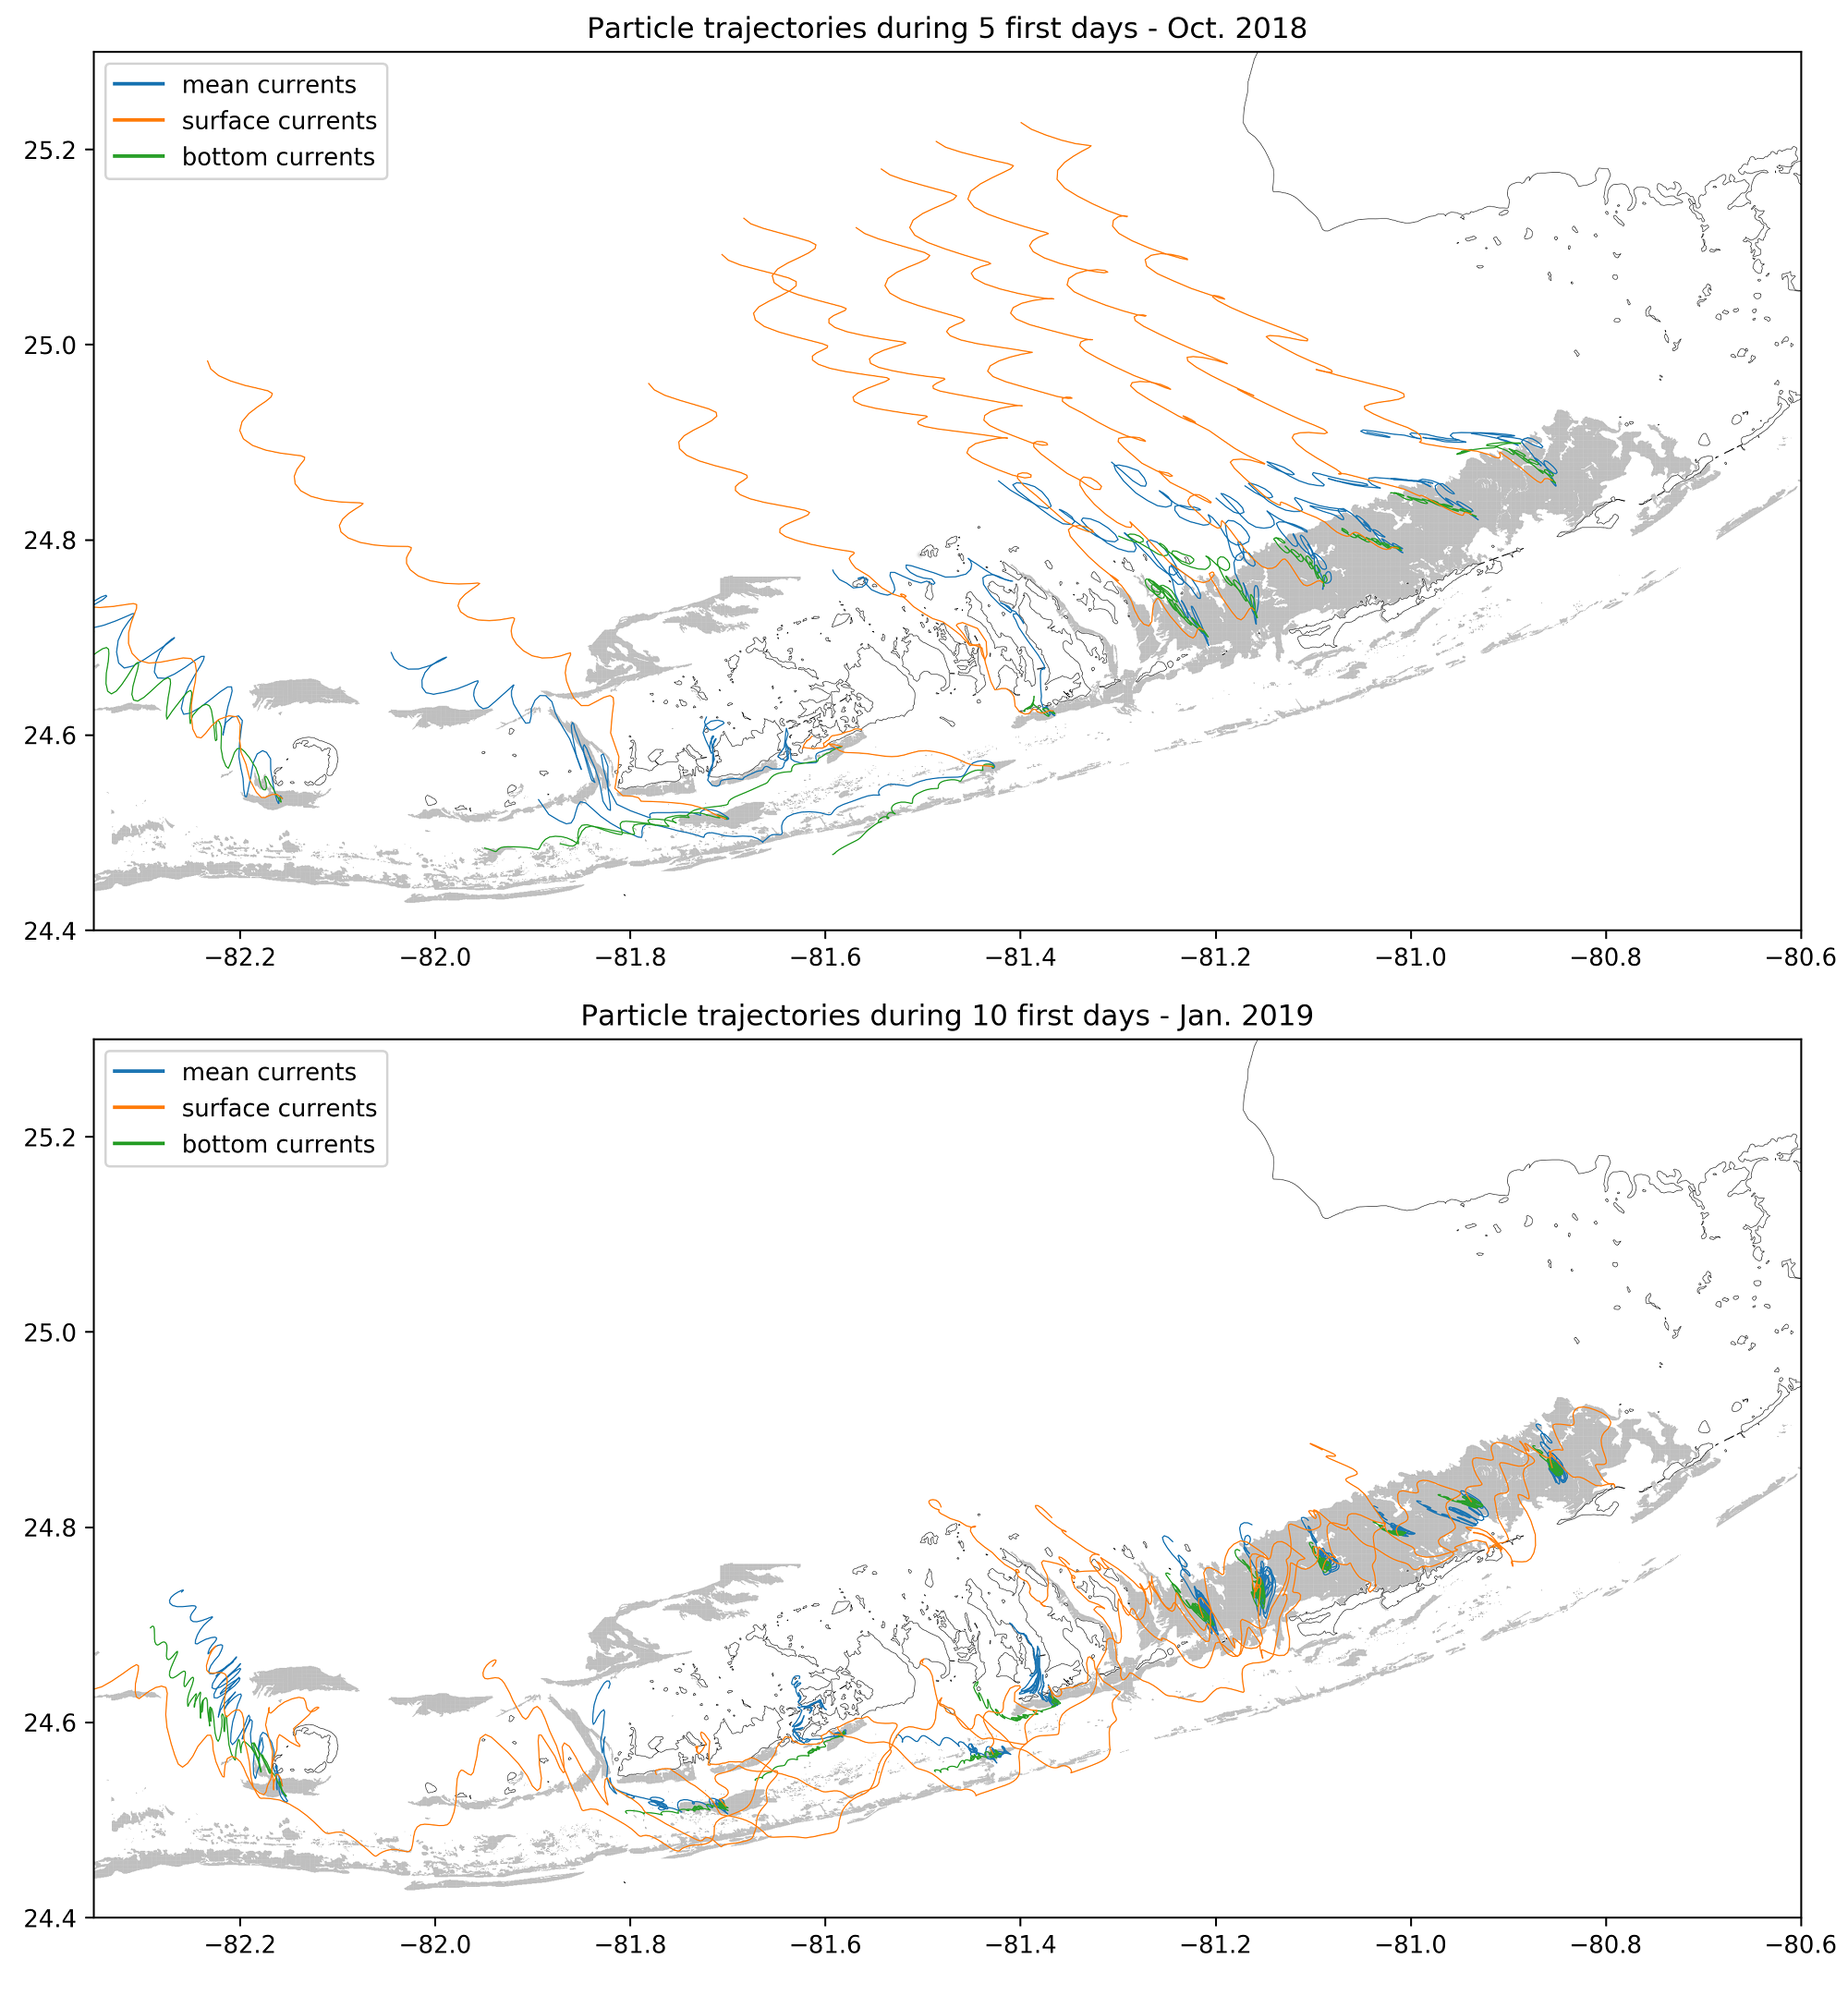
\includegraphics[width=.9\textwidth]{figures/traj.png}
%     \caption{}
%     \label{fig:traj}
% \end{figure}

%\begin{figure}[h]
%    \centering
%    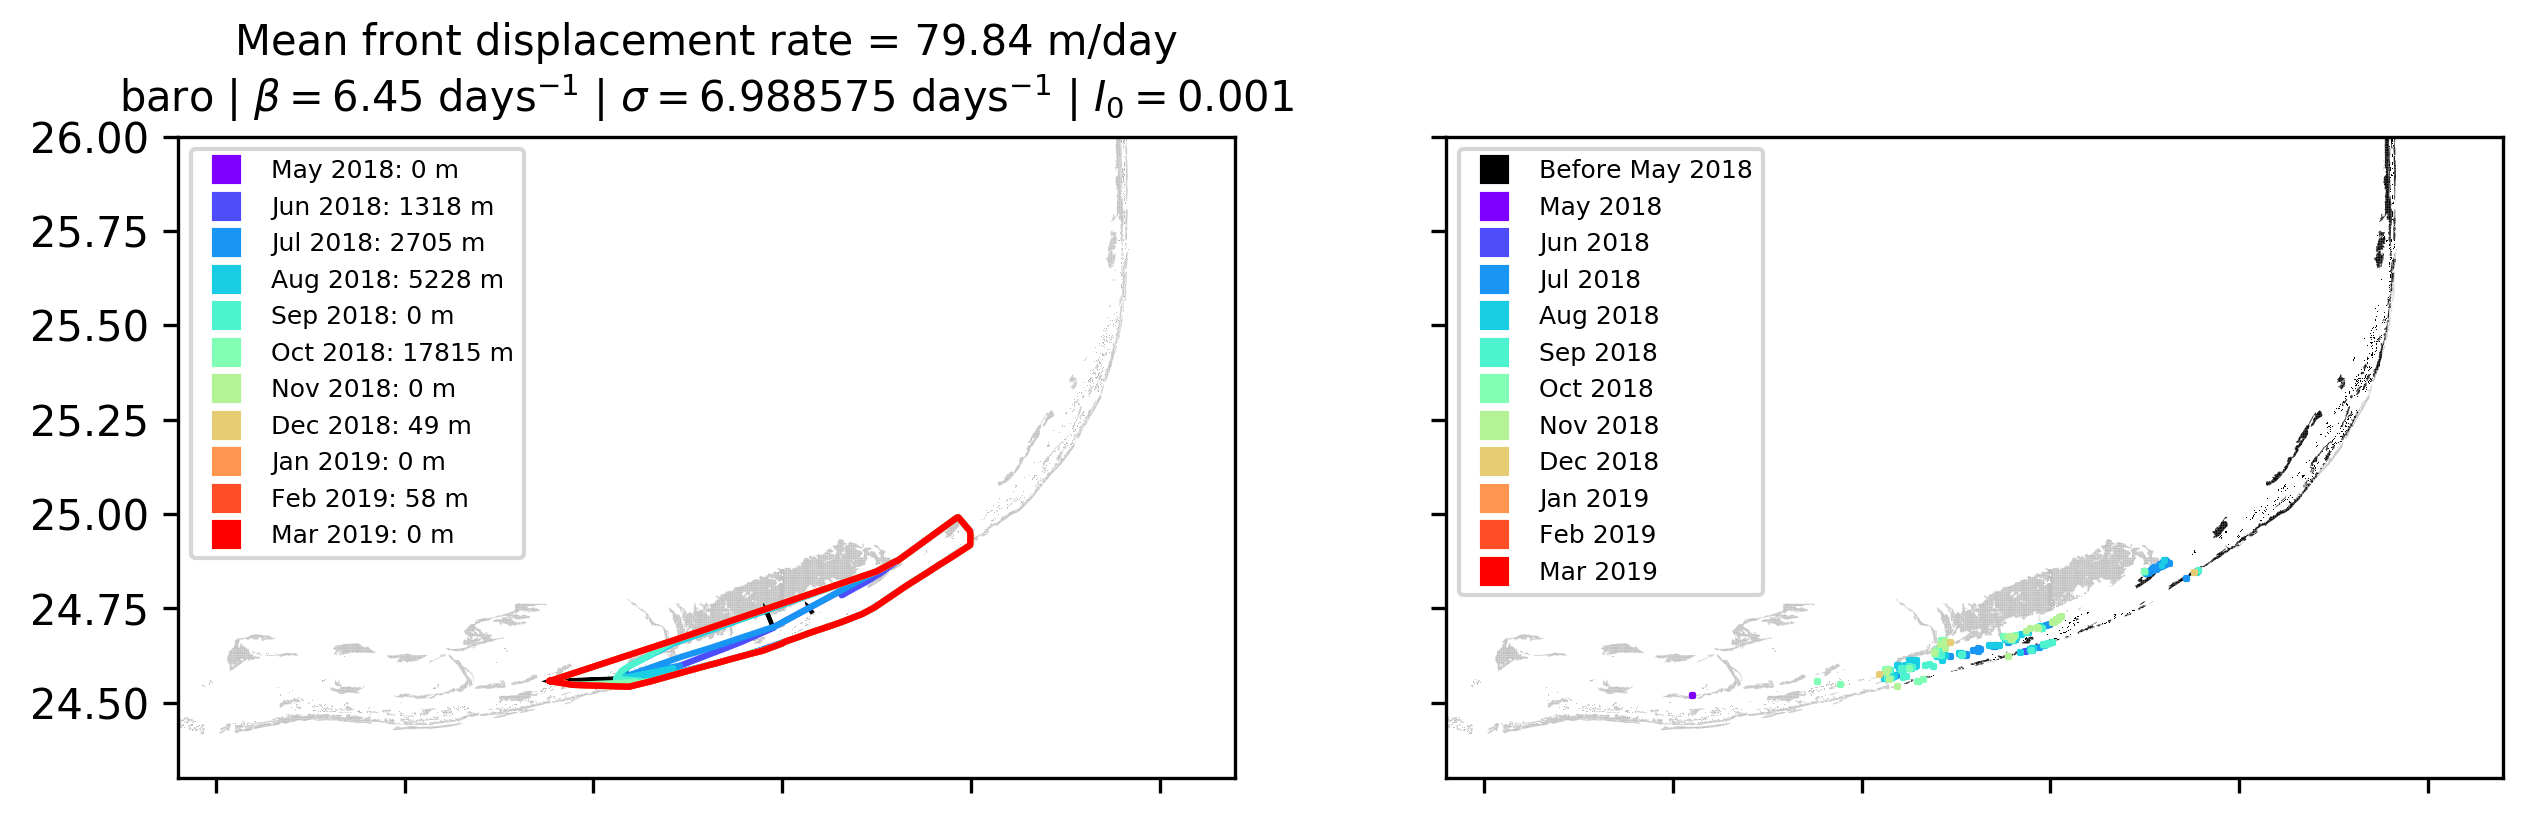
\includegraphics[width=.9\textwidth]{figures/hull_result.png}
%    \caption{Take home messages:\begin{itemize}
%        \item Our methods accurately captures disease front evolution through time (mtch between points and concave hulls)
%    \end{itemize}}
%    \label{fig:front}
%\end{figure}

% === DISCUSSION === %
\section{Discussion and conclusions}

%% --- SUMMARY OF TAKE HOME MESSAGES --- %%

We have developed an epidemio-hydrodynamic model to simulate the spread of the SCTLD through the entire FRT. Calibrating our model with colonies-averaged prevalence observations, we estimate the species-averaged reproduction number to be slightly above 1. Feeding this parameter to the model, our simulation suggest that only mean current are able to reproduce the observed spread o the disease. Bottom current do not spread infectious matter on a sufficient geographical range while surface currents do not allow infected elements to settle durably on reefs. The causative agent of the SCTLD is therefore expected to be transported within neutrally buoyant materials inside the water column. Assuming this mode of transport, propagation of the disease from reef to reef only occurs for a narrow range of values of infection threshold $I_0$. This threshold is defined as the proportion of colonies that have to be infected to trigger an exponential increase of the disease on a reef. As disease spread occurs for threshold values of in the range $0.05-0.1\%$, this suggests that corals have low resistance to the SCTLD.

%% --- DISCUSSION OF TAKE HOME MESSAGES/MAIN RESULTS --- %%

% 1. MODEL PARAMETERS
After calibration, we estimated the species-averaged basic reproduction number $\beta_0'/\sigma$ to be equal to $1.0835$. This value being close to 1, modeled infectious individuals are removed from the system almost as fast as susceptible individuals get infected. This causes the proportion of infectious corals on the reefs to remain pretty low (\ie $\leq 0.4\%$) through time. This suggests that only a small fraction of the colony causes the disease to spread on the reef during the outbreak. \erinn{[add some comments on tank experiments + comparison with model results]}. In this study, the same values were used for inter- and intra-reef rates $\beta$ and $\beta_0'$. This implies that the infectiousness of the causative agent is not reduced during its journey from reef to reef. However, to assess the impact of this assumption, epidemiological model simulations were performed with $\beta=\beta_0'/2$. The resulting disease front speeds did not exceed 20 m/day. This strong decrease can be explained by the interplay between inter- and intra- reef infection. Reducing inter-reef transmission rates decreases the proportion of infectious corals on reefs attained by infectious materials, which in turn reduces the amount of infectious matter sent to the rest of the network. This suggests that, to reproduce the observed spread, inter- and intra-reef transmission rates must have similar magnitude, \ie that the causative agent is barely not degraded while traveling from reef to reef. \dobby{Is this consistent with Rhodobacterales and Rhizobiales ?}

% 2. MEAN BAROTROPIC CURRENTS => NEUTRALLY BUOYANT VECTOR 

The fact that mean barotropic currents outperform the other modes of transport in \ref{fig:results} can be explained by considering the trajectories of the particles used to model the transport of the vector of the disease causative agent. Due to the impact of winds on positively buoyant materials, particles driven by surface currents are likely to be blown away from the reefs. Moreover, even when winds are pushing particles along the reef line, these particles spend less time over the same region than particles driven by mean and bottom currents. Smaller amounts of particle mass will therefore settle on reef polygons, leading to lower entries of the potential connectivity matrix, \ie lower exchange probabilities between reefs. Hence, despite being able to displace infected materials on greater distances, surface currents are less likely to drive the propagation of the disease. Particles driven by bottom currents, on the other hand, remain longer over the same region, producing larger entries of the potential connectivity matrix. Due to these large exchange probabilities between reefs, bottom currents are better at propagating the disease (Fig. \ref{fig:results}). Nevertheless, bottom currents being relatively slower, exchanges of infected materials occur on a limited geographical range. Mean barotropic currents, that carry particles on greater distances while allowing for sufficiently large amounts of infected mass to settle on reef polygons, are thus best suited to propagate the disease (Fig. \ref{fig:results}).

Since mean currents are the only mode of transport that successfully reproduces the observed propagation speed of the disease in our model, the disease causative agent is expected to be transported within neutrally buoyant material inside the water column. This assumption seems reasonable as water-borne transmission is implicated as an important spreading mechanism for multiple coral diseases, including white band disease, white plague disease, white pox disease, white syndrome disease, \textit{Porites} ulcerative white spots diseases, skeletal eroding band disease \citep{shore2019modes}. \dobby{[examples of neutrally buoyant vectors ? mucus ?]}. The causative agent might also be transported within fine sediments such as silt, as suggested by \cite{rosales2020rhodobacterales}. Such sediments are easily eroded in shallow areas around coral reefs and would therefore be mostly transported inside the water column by mean barotropic currents. This hypothesis might be tested by adapting the deposition rate $\gamma$ used in our experiments to be consistent with the sedimentation rate of silt. However, such modification of $\gamma$ would alter the entries of our potential connectivity matrices. Nonetheless, the sensitivity of the connectivity matrices to the value of $\gamma$ has been briefly assessed by generating new matrices using particles with a half-life of 15 days ($\gamma$ increased by a factor two). Although these matrices exhibited stronger short-range connectivity, the impact on connectivity indicator values remained  limited ($<10\%$). This suggests that the main results of this study would remain valid for fine sediments.  

%  * Talk about ballast waters study (bottom currents) (?)
%  * most susceptible species not branching corals. Quite surprising as branching/corals with folioses moe susceptible to water-borne transmission :-( 

% 3. IMPACT OF I0/APPEARANCE OF PLATEAU
Coral resistance to the SCTLD in represented by parameter $I_0$, defined as the maximum proportion of the colony that can get infected without causing the disease to spread to the rest of the colony. The modeled propagation of the disease is highly sensitive to this parameter. On the one hand, when corals are strongly susceptible to the disease, infectious individuals are removed from the system too fast to become sustainable sources of infectious materials in the network. On the other hand, if corals are weakly susceptible to the disease, very few corals get infected and the disease barely propagates. Our simulations suggest that this value must be fairly low (around 0.01\%) in order to successfully spread the disease throughout the FRT. \dobby{This seems to imply that susceptible coral species have very weak defense mechanisms against the causative agent of the disease. (?)}.\\
% \dobby{TO DO: link $I_0$ to pathogenic load}\\
% \noindent\fbox{%
%     \parbox{.95\linewidth}{%
%         Let $T$ be the time at which the proportion of infectious individuals $I_j$ attains $I_0$ on reef $j$. The cumulative quantity of infectious materials that reached reef $j$ at time $T$ (= proxy of infectious load) is given by 
%         \begin{equation}
%             \beta\sum_i\dfrac{A_i}{A_j}\tilde{C}_{ij}\int_0^T I_i(t)dt
%         \end{equation}
%         The larger $I_0$, the larger the pathogen load before intra-reef propagation occurs (transition water-borne to direct transmission)
%     }%
% }

%% --- LIMITATION AND POTENTIAL IMPROVEMENTS OF THE MODEL --- %%
% 1. Limitations of hydro
As with any modeling study, it is important to understand the assumptions on which the model is based. Here, we have used a 2D barotropic ocean model coupled with the 3D model HYCOM \citep{Chassignet2007} in order to indirectly represent baroclinic phenomena. Such model is well suited to simulate the fate of neutrally-buoyant matters in shallow regions. However, as depth-averaged currents do not accurately approximate the motion of particles in the bottom and surface layers, \slim velocities have been modified to simulate the exchanges of negatively and positively buoyant matters. Surface current response to wind parametrization is based on the results of \cite{ardhuin2009observation}, consistent with observations. In this study, measured surface currents are shown to be in the order of $1.0\% - 1.8\%$ of the wind speed, in a direction $10^\circ - 40^\circ$ to the right of the wind. \lew{[discuss bottom currents parametrization]}. Although such estimation of surface and bottom currents is disputable, using a 2D model allows for reef-scale resolution throughout the whole FRT. Such high-resolution allows to capture recirculation eddies around islands and reefs, that significantly impact the weighted connectivity length as well as the local retention on the reefs.

% 2. Limitations of epidemiological model
The appearance of an interval of optimal values of threshold $I_0$ for the propagation of the disease in our results highlights the impact of coral resistance on the spread of SCTLD through the FRT. Therefore, a further step in our modeling approach would be further dividing coral populations of our polygons into highly susceptible (\eg \textit{Dichocoenia stokesii}, \textit{Meandrina meandrites}), intermediately susceptible (\eg \textit{Orbicella faveolata}, \textit{Montastrea cavernosa}), and weakly susceptible (\eg \textit{Acropora Palmata}, \textit{Acropora cervicornis}) sub-populations. The proportions susceptible, infectious and removed individuals within these sub-populations would then be modeled with specific transmission ($\beta$, $\beta_0'$) and removal ($\sigma$) rates as well as specific infection thresholds $I_0$. Such approach would however require a fine knowledge of the distribution of the different coral species throughout the FRT. This knowledge about coral coverage could also be used to avoid overestimation of the front propagation, as in the case of Vaca reef.

%% --- NICE FINAL PARAGRAPH --- %%
Despite the limitations of its current formulation, we believe that our model brings unprecedented perspectives on the propagation mechanism of the SCTLD through the FRT. Using a reef-scale spatial resolution, we determined the most probable mode of transport for the vector of the disease agent and deduced its species-averaged reproduction number based on prevalence observations. Besides, our model formulation provides a framework to quantity coral resistance to the disease. As our model results are continuous through time, they can exhibit the variability of the propagation of the SCTLD through time and therefore bring additional insight to observation data. This study therefore provides much-needed complementary insight on the identification of the causative agent of the Stony Coral Tissue Loss disease and the management of the crisis it generates.

% === APPENDIX === %
%\appendix
\section*{Appendix}

% --- MODEL FORMULATION --- %   
\subsection*{Subsection 1}
% --- MODEL EVALUATION --- %
\subsection*{Subsection 2}

\section*{Conflict of Interest Statement}
The authors declare that the research was conducted in the absence of any commercial or financial relationships that could be construed as a potential conflict of interest.

\section*{Author Contributions}
  
\section*{Funding}
This paper is a result of research funded by the Florida Department of Environmental Protection under award XXX to Mote Marine Laboratory. 

\section*{Acknowledgments}
Computational resources were provided by the Consortium des \'Equipements de Calcul Intensif (\textsc{c\'eci}), funded by the \textsc{f.r.s.-fnrs} under Grant No. 2.5020.11.

\section*{Supplemental Data}

% === BIBLIOGRAPHY === %
\bibliographystyle{frontiersinSCNS_ENG_HUMS} 
\bibliography{./biblio.bib}

%%% Make sure to upload the bib file along with the tex file and PDF
%%% Please see the test.bib file for some examples of references

\section*{Tables and figures}


\end{document}
